% ===========================================================================
%  MEng Dissertation — Implementation Strategies for Defending Against Evasion Attacks in Adversarial Machine Learning on IoMT Data
%  National Higher Polytechnic Institute (NAHPI)
%  The University of Bamenda, Cameroon
% ===========================================================================

\documentclass[12pt,a4paper,oneside]{report}

% ---------------------------------------------------------------------------
% Packages
% ---------------------------------------------------------------------------
\usepackage[utf8]{inputenc}
\usepackage[T1]{fontenc}
\usepackage{times}
\usepackage{setspace}
\usepackage[margin=2.5cm, left=3.5cm, right=2.5cm]{geometry}
\usepackage{graphicx}
\usepackage{float}
\usepackage{caption}
\usepackage{amsmath,amssymb}
\usepackage{booktabs}
\usepackage{longtable}
\usepackage{array}
\usepackage{hyperref}
\usepackage{enumitem}
\usepackage{multirow}
\usepackage{fancyhdr}
\usepackage{tocloft}
\usepackage{appendix}
\usepackage{xcolor}
\usepackage{listings}
\usepackage{textcomp}


% ---------------------------------------------------------------------------
% Page style
% ---------------------------------------------------------------------------
\pagestyle{fancy}
\fancyhf{}
\fancyfoot[C]{\thepage}
\renewcommand{\headrulewidth}{0pt}
\renewcommand{\footrulewidth}{0pt}

\onehalfspacing
\setlength{\parindent}{1.27cm}
\graphicspath{{../reports/}{./figures/}{./appendix/}}

\hypersetup{
    colorlinks=true,
    linkcolor=black,
    citecolor=black,
    urlcolor=blue,
}

\setcounter{tocdepth}{3}
\setcounter{secnumdepth}{3}

\newcommand{\reffig}[1]{Figure~\ref{#1}}
\newcommand{\reftab}[1]{Table~\ref{#1}}
\newcommand{\refeq}[1]{Equation~\ref{#1}}

% ===========================================================================
\begin{document}

% ---------------------------------------------------------------------------
% PRELIMINARY PAGES
% ---------------------------------------------------------------------------
\pagenumbering{roman}

% === Cover page ===
\thispagestyle{empty}
\begin{center}
    \vspace*{0.5cm}
    {\large REPUBLIC OF CAMEROON}\\[0.2cm]
    {\large Peace---Work---Fatherland}\\[0.5cm]
    \rule{\textwidth}{0.5pt}\\[0.3cm]
    {\Large THE UNIVERSITY OF BAMENDA}\\[0.2cm]
    {\Large NATIONAL HIGHER POLYTECHNIC INSTITUTE}\\[0.2cm]
    {\large Department of Computer Engineering}\\[1.5cm]
    \rule{\textwidth}{0.5pt}\\[0.8cm]
    {\Huge\bfseries Implementation Strategies for Defending Against Evasion Attacks in Adversarial Machine Learning on IoMT Data}\\[1.0cm]
    \rule{\textwidth}{0.5pt}\\[1.0cm]
    {\large A Dissertation Submitted to the Department of Computer Engineering}\\
    {\large in the National Higher Polytechnic Institute of}\\
    {\large The University of Bamenda in Partial Fulfillment}\\
    {\large of the Requirements for the Award of a}\\[0.3cm]
    {\Large\bfseries Master of Engineering (MEng) Degree in Computer Engineering}\\[1.0cm]
    {\large Option: Software Engineering}\\[1.5cm]
    {\large\bfseries BY:}\\[0.3cm]
    {\Large MALWARE XXXXXXXX XXXXXXXXX}\\[0.2cm]
    {\large Registration Number: XX-XXXX-XX}\\[1.5cm]
    {\large\bfseries SUPERVISOR:}\\[0.3cm]
    {\large Dr. XXXXXX XXXXXXXX}\\[0.2cm]
    {\large (Senior Lecturer)}\\[1.5cm]
    {\large\bfseries CO-SUPERVISOR:}\\[0.3cm]
    {\large Engr. XXXXXX XXXXXXXX}\\[0.2cm]
    {\large (Assistant Lecturer)}\\[1.5cm]
    {\large Month, Year}
    \vfill
\end{center}
\newpage

% === Title page ===
\thispagestyle{empty}
\begin{center}
    \vspace*{0.5cm}
    {\large REPUBLIC OF CAMEROON}\\[0.2cm]
    {\large Peace---Work---Fatherland}\\[0.5cm]
    \rule{\textwidth}{0.5pt}\\[0.3cm]
    {\Large THE UNIVERSITY OF BAMENDA}\\[0.2cm]
    {\Large NATIONAL HIGHER POLYTECHNIC INSTITUTE}\\[0.2cm]
    {\large Department of Computer Engineering}\\[1.5cm]
    \rule{\textwidth}{0.5pt}\\[0.8cm]
    {\Huge\bfseries Implementation Strategies for Defending Against Evasion Attacks in Adversarial Machine Learning on IoMT Data}\\[1.0cm]
    \rule{\textwidth}{0.5pt}\\[1.0cm]
    {\large A Dissertation Submitted to the Department of Computer Engineering}\\
    {\large in the National Higher Polytechnic Institute of}\\
    {\large The University of Bamenda in Partial Fulfillment}\\
    {\large of the Requirements for the Award of a}\\[0.3cm]
    {\Large\bfseries Master of Engineering (MEng) Degree in Computer Engineering}\\[1.0cm]
    {\large Option: Software Engineering}\\[1.5cm]
    {\large\bfseries BY:}\\[0.3cm]
    {\Large MALWARE XXXXXXXX XXXXXXXXX}\\[0.2cm]
    {\large Registration Number: XX-XXXX-XX}\\[1.5cm]
    {\large\bfseries SUPERVISOR:}\\[0.3cm]
    {\large Dr. XXXXXX XXXXXXXX}\\[0.2cm]
    {\large (Senior Lecturer)}\\[0.5cm]
    {\large\bfseries CO-SUPERVISOR:}\\[0.3cm]
    {\large Engr. XXXXXX XXXXXXXX}\\[0.2cm]
    {\large (Assistant Lecturer)}\\[1.5cm]
    {\large Month, Year}
    \vfill
\end{center}
\newpage

% === Copyright page ===
\thispagestyle{empty}
\begin{center}
    \vspace*{4cm}
    {\large\bfseries \copyright~Copyright by MALWARE XXXXXXXX XXXXXXXXX, Year}\\[0.5cm]
    {\large All rights reserved}
    \vfill
\end{center}
\newpage

% === Declaration page ===
\thispagestyle{empty}
\begin{center}
    {\Large\bfseries DECLARATION OF ORIGINALITY OF STUDY}
\end{center}
\vspace{1cm}

I, \textbf{MALWARE XXXXXXXX XXXXXXXXX}, Registration Number: \textbf{XX-XXXX-XX}, in the Department of \textbf{Computer Engineering}, National Higher Polytechnic Institute, The University of Bamenda hereby declare that this work titled \textbf{``Implementation Strategies for Defending Against Evasion Attacks in Adversarial Machine Learning on IoMT Data''} is my original work. It has not been presented in any application for a degree or any academic pursuit elsewhere. I have acknowledged all borrowed ideas nationally and internationally through citations.

\vspace{2cm}

\noindent Date:~\rule{5cm}{0.4pt}\hfill Signature of author:~\rule{5cm}{0.4pt}
\vfill
\newpage

% === Acceptance page (MEng only) ===
\thispagestyle{empty}
\begin{center}
    {\Large\bfseries ACCEPTANCE OF DISSERTATION}
\end{center}
\vspace{1cm}

Having met the stipulated requirements, this dissertation entitled \textbf{``Implementation Strategies for Defending Against Evasion Attacks in Adversarial Machine Learning on IoMT Data''} has been accepted by the Postgraduate School of The University of Bamenda in partial fulfillment of the requirements for the award of a \textbf{Master of Engineering (MEng) Degree in Computer Engineering} (Option: Software Engineering).

\vspace{2cm}

\begin{flushleft}
Chairperson, Master's Dissertation Committee:\hrulefill\\[0.3cm]
Prof.~XXXXXX XXXXXXXX\\[1cm]
Date:~\rule{5cm}{0.4pt}
\end{flushleft}
\vfill
\newpage

% === Abstract (English) ===
\thispagestyle{empty}
\begin{center}
    {\Large\bfseries ABSTRACT}
\end{center}
\vspace{0.5cm}

The rapid proliferation of Internet of Medical Things (IoMT) devices in healthcare has created an urgent need for robust machine learning models capable of detecting cyber threats while resisting adversarial manipulation. This study addresses the vulnerability of machine learning classifiers to evasion attacks, where adversaries deliberately craft small perturbations to input data to cause misclassification. The research implements and evaluates four defense strategies---adversarial training, feature selection, ensemble methods, and feature squeezing---against two prominent evasion attacks, namely the Fast Gradient Sign Method (FGSM) and Projected Gradient Descent (PGD), on the CIC\_IoMT\_2024 dataset. Three base classifiers were employed: Random Forest, XGBoost, and LightGBM. Experimental results demonstrate that XGBoost achieved the highest clean accuracy of 93.70\% and F1 score of 93.63\%, while LightGBM exhibited the lowest performance at 57.27\% accuracy. Without defense, model accuracy on FGSM-attacked data at $\epsilon = 0.01$ dropped from 93.70\% to 18.38\%, confirming the severe impact of evasion attacks. Among the defenses evaluated, adversarial training provided the most balanced robustness, maintaining accuracies between 26.03\% and 38.03\% across epsilon values. Feature selection alone was insufficient, reducing accuracy to 16.34\% even on clean data due to excessive feature removal. The ensemble defense preserved the highest clean accuracy (84.95\%) but degraded rapidly under attack. These findings underscore the critical importance of selecting appropriate defense mechanisms for IoMT security applications and provide a quantitative framework for evaluating defense strategies against adversarial threats in healthcare environments.

\vspace{0.5cm}
\noindent\textbf{Keywords:} Adversarial Machine Learning, Evasion Attacks, IoMT Security, Defense Strategies, FGSM, PGD, Random Forest, XGBoost, LightGBM
\newpage

% === Resume (French) ===
\thispagestyle{empty}
\begin{center}
    {\Large\bfseries R\'ESUM\'E}
\end{center}
\vspace{0.5cm}

La prolif\'eration rapide des dispositifs Internet des Objets M\'edicaux (IoMT) dans le domaine de la sant\'e a cr\'e\'e un besoin urgent de mod\`eles d'apprentissage automatique robustes capables de d\'etecter les cybermenaces tout en r\'esistant \`a la manipulation adversarial. Cette \'etude aborde la vuln\'erabilit\'e des classifieurs d'apprentissage automatique aux attaques par \'evasion, o\`u les adversaires cr\'eent d\'elib\'er\'ement de petites perturbations dans les donn\'ees d'entr\'ee pour provoquer une mauvaise classification. La recherche impl\'emente et \'evalue quatre strat\'egies de d\'efense---l'entra\^inement adversarial, la s\'election de caract\'eristiques, les m\'ethodes d'ensemble, et la compression des caract\'eristiques---contre deux attaques par \'evasion importantes, \`a savoir la M\'ethode du Signe du Gradient Rapide (FGSM) et la Descente de Gradient Projet\'ee (PGD), sur l'ensemble de donn\'ees CIC\_IoMT\_2024. Trois classifieurs de base ont \'et\'e employ\'es : For\^et Al\'eatoire, XGBoost et LightGBM. Les r\'esultats exp\'erimentaux d\'emontrent que XGBoost a atteint la pr\'ecision propre la plus \'elev\'ee de 93.70\% et un score F1 de 93.63\%, tandis que LightGBM a pr\'esent\'e la performance la plus faible avec une pr\'ecision de 57.27\%. Sans d\'efense, la pr\'ecision du mod\`ele sur les donn\'ees attaqu\'ees par FGSM \`a $\epsilon = 0.01$ est pass\'ee de 93.70\% \`a 18.38\%, confirmant l'impact s\'ev\`ere des attaques par \'evasion. Parmi les d\'efenses \'evalu\'ees, l'entra\^inement adversarial a fourni la robustesse la plus \'equilibr\'ee, maintenant des pr\'ecisions entre 26.03\% et 38.03\% pour toutes les valeurs d'epsilon. La s\'election de caract\'eristiques seule \'etait insuffisante, r\'eduisant la pr\'ecision \`a 16.34\% m\^eme sur des donn\'ees propres en raison d'un retrait excessif de caract\'eristiques. La d\'efense d'ensemble a pr\'eserv\'e la pr\'ecision propre la plus \'elev\'ee (84.95\%) mais s'est d\'egrad\'ee rapidement sous attaque. Ces r\'esultats soulignent l'importance cruciale de s\'electionner des m\'ecanismes de d\'efense appropri\'es pour les applications de s\'ecurit\'e IoMT et fournissent un cadre quantitatif pour \'evaluer les strat\'egies de d\'efense contre les menaces adversariales dans les environnements de soins de sant\'e.

\vspace{0.5cm}
\noindent\textbf{Mots-cl\'es:} Apprentissage Automatique Adversarial, Attaques par \'Evasion, S\'ecurit\'e IoMT, Strat\'egies de D\'efense, FGSM, PGD, For\^et Al\'eatoire, XGBoost, LightGBM
\newpage

% === Dedication ===
\thispagestyle{empty}
\begin{center}
    {\Large\bfseries DEDICATION}
\end{center}
\vspace{1cm}

To my family, for their unwavering support and encouragement throughout this journey.

\vfill
\newpage

% === Acknowledgment ===
\thispagestyle{empty}
\begin{center}
    {\Large\bfseries ACKNOWLEDGMENT}
\end{center}
\vspace{0.5cm}

I wish to express my profound gratitude to my supervisor, Dr.~XXXXXX XXXXXXXX, for his invaluable guidance, patience, and constructive criticism throughout this research. His expertise and mentorship have been instrumental in shaping this work.

I am equally grateful to my co-supervisor, Engr.~XXXXXX XXXXXXXX, for his technical insights and continuous support.

My sincere appreciation goes to the Head of Department of Computer Engineering and all the lecturers who imparted knowledge and skills that contributed to the successful completion of this dissertation.

I also acknowledge the support of my classmates and friends, whose encouragement and collaboration made this journey memorable.

Above all, I thank the Almighty God for His grace and strength throughout this academic pursuit.

\vfill
\newpage

% === Table of Contents ===
\thispagestyle{empty}
\begin{center}
    {\Large\bfseries TABLE OF CONTENTS}
\end{center}
\vspace{0.5cm}
\tableofcontents
\newpage

% === List of Tables ===
\thispagestyle{empty}
\begin{center}
    {\Large\bfseries LIST OF TABLES}
\end{center}
\vspace{0.5cm}
\listoftables
\newpage

% === List of Figures ===
\thispagestyle{empty}
\begin{center}
    {\Large\bfseries LIST OF FIGURES}
\end{center}
\vspace{0.5cm}
\listoffigures
\newpage

% === List of Abbreviations ===
\thispagestyle{empty}
\begin{center}
    {\Large\bfseries LIST OF ABBREVIATIONS}
\end{center}
\vspace{0.5cm}

\begin{longtable}{p{4cm} p{10cm}}
\textbf{Abbreviation} & \textbf{Full Meaning} \\
\midrule
\endhead
AML    & Adversarial Machine Learning \\
API    & Application Programming Interface \\
ASR    & Attack Success Rate \\
CIC    & Canadian Institute for Cybersecurity \\
FGSM   & Fast Gradient Sign Method \\
FN     & False Negative \\
FP     & False Positive \\
GAN    & Generative Adversarial Network \\
IoMT   & Internet of Medical Things \\
LGBM   & Light Gradient Boosting Machine \\
MEng   & Master of Engineering \\
ML     & Machine Learning \\
NAHPI  & National Higher Polytechnic Institute \\
PGD    & Projected Gradient Descent \\
RAM    & Random Access Memory \\
RF     & Random Forest \\
ROC-AUC & Receiver Operating Characteristic --- Area Under the Curve \\
SHAP   & SHapley Additive exPlanations \\
TN     & True Negative \\
TP     & True Positive \\
UBa    & University of Bamenda \\
XGB    & XGBoost (Extreme Gradient Boosting) \\
\end{longtable}
\newpage

% ===========================================================================
%  MAIN BODY
% ===========================================================================
\pagenumbering{arabic}

% ===================================================================
%  CHAPTER 1: INTRODUCTION
% ===================================================================
\chapter{INTRODUCTION}

\section{Background and Statement of the Problem}

The rapid digitisation of healthcare systems has led to the widespread adoption of Internet of Medical Things (IoMT) devices, including smart sensors, wearable monitors, and connected diagnostic equipment. These devices generate vast quantities of sensitive medical data that must be processed and analysed in real time to support clinical decision-making. Machine learning (ML) models have become indispensable tools for analysing IoMT data, enabling applications such as intrusion detection, anomaly detection, and predictive diagnosis \cite{goodfellow2015explaining}.

Despite their effectiveness, ML models are inherently vulnerable to adversarial attacks. An adversary can introduce carefully crafted perturbations to input data that are imperceptible to humans but cause the model to make incorrect predictions. These attacks, known as evasion attacks, pose a critical threat to IoMT systems where misclassification could lead to misdiagnosis, delayed treatment, or failure to detect malicious activity \cite{madry2018towards, papernot2016limitations}.

The Fast Gradient Sign Method (FGSM), introduced by Goodfellow et al.~\cite{goodfellow2015explaining}, is a single-step attack that perturbs each feature in the direction that maximally increases the loss function. The Projected Gradient Descent (PGD) method, proposed by Madry et al.~\cite{madry2018towards}, extends FGSM by taking multiple smaller steps while projecting the perturbation back onto an epsilon-ball, producing stronger adversarial examples.

The CIC\_IoMT\_2024 dataset, published by the Canadian Institute for Cybersecurity, comprises network traffic data from IoMT devices across 51 classes of normal and attack traffic. This dataset provides a realistic and challenging testbed for evaluating ML-based intrusion detection systems and their vulnerability to adversarial manipulation.

The problem addressed by this research is the vulnerability of ML classifiers to evasion attacks in the IoMT domain. Without adequate defenses, an adversary can degrade model performance dramatically---for instance, reducing accuracy from over 93\% to below 20\% with minimal perturbations. This study investigates four defense strategies to mitigate these vulnerabilities and quantifies their effectiveness through systematic experimentation.

\section{Rationale}

The rationale for this study stems from the critical need to secure IoMT systems against adversarial threats. Healthcare environments present unique challenges: the data is high-dimensional, multi-class, and imbalanced; the cost of misclassification can be life-threatening; and the computational resources available for defense may be constrained.

Previous research has predominantly focused on adversarial attacks and defenses in the image domain, where pixel values have natural bounds and gradient-based attacks are straightforward to implement. Tabular data, which is the primary format of IoMT network traffic, presents different challenges. Tree-based ensemble models such as Random Forest, XGBoost, and LightGBM---which are widely used in tabular domains---do not provide smooth gradients, requiring adaptations of gradient-based attacks.

This research addresses the gap by implementing and evaluating four defense strategies specifically adapted for tabular data and tree-based models. The study provides a quantitative comparison that can guide practitioners in selecting appropriate defenses for IoMT security applications.

\section{Research Questions}

\subsection{Main Research Question}

How effective are adversarial training, feature selection, ensemble methods, and feature squeezing at mitigating evasion attacks (FGSM and PGD) on tree-based machine learning classifiers trained on IoMT network traffic data?

\subsection{Specific Research Questions}

\begin{enumerate}[label=\textbf{RQ\arabic*:}]
    \item What is the baseline clean performance of Random Forest, XGBoost, and LightGBM classifiers on the CIC\_IoMT\_2024 dataset in terms of accuracy, precision, recall, and F1 score?
    \item How severely do FGSM and PGD attacks degrade the performance of each classifier across varying perturbation magnitudes?
    \item Which defense strategy provides the greatest improvement in robustness, measured as the accuracy maintained on adversarially perturbed data?
    \item How does the complexity and computational cost of each defense strategy compare to its robustness benefit?
\end{enumerate}

\section{Objectives}

\subsection{Overall Objective}

The overall objective of this study was to implement and evaluate defense strategies against evasion attacks in adversarial machine learning on IoMT data.

\subsection{Specific Objectives}

The specific objectives were:

\begin{enumerate}
    \item To implement a data pipeline for loading, cleaning, and preprocessing the CIC\_IoMT\_2024 dataset;
    \item To train and evaluate three base classifiers---Random Forest, XGBoost, and LightGBM---on the preprocessed dataset;
    \item To implement FGSM and PGD evasion attacks adapted for tree-based models;
    \item To implement four defense strategies: adversarial training, feature selection, ensemble methods, and feature squeezing;
    \item To evaluate and compare the effectiveness of each defense strategy using quantitative metrics.
\end{enumerate}


% ===================================================================
%  CHAPTER 2: LITERATURE REVIEW
% ===================================================================
\chapter{LITERATURE REVIEW}

\section{Overview of Adversarial Machine Learning}

Adversarial machine learning is a subfield of artificial intelligence that studies the vulnerability of ML models to malicious inputs and develops techniques to make models more robust. The field emerged from the observation that neural networks are susceptible to small, intentional perturbations of input data that cause misclassification with high confidence \cite{szegedy2013intriguing}. Since then, research has expanded to cover a wide range of model architectures, attack types, and application domains.

Adversarial attacks can be categorised along several dimensions. \textbf{By attacker knowledge:} white-box attacks assume full knowledge of the model architecture and parameters, while black-box attacks assume no internal knowledge. \textbf{By attack goal:} targeted attacks aim to cause misclassification to a specific class, while untargeted attacks aim to cause any misclassification. \textbf{By attack timing:} poisoning attacks corrupt training data, while evasion attacks manipulate inputs at inference time \cite{biggio2013evasion}.

This study focuses on white-box evasion attacks, where the adversary has access to the model's parameters and can compute perturbation directions during inference.

\section{Evasion Attacks}

Evasion attacks generate adversarial examples---inputs that are intentionally modified to cause misclassification while appearing legitimate to human observers. The mathematical formulation of an evasion attack can be expressed as an optimisation problem:

\begin{equation}
    \label{eq:evasion}
    \max_{\|\delta\|_p \leq \epsilon} \mathcal{L}(f(x + \delta), y)
\end{equation}

\noindent where $x$ is the original input, $y$ is the true label, $f$ is the classifier, $\mathcal{L}$ is the loss function, $\delta$ is the perturbation vector, $\epsilon$ bounds the perturbation magnitude in the $\ell_p$ norm, and the goal is to maximise the loss.

\subsection{Fast Gradient Sign Method (FGSM)}

The Fast Gradient Sign Method, introduced by Goodfellow et al.~\cite{goodfellow2015explaining}, is a single-step attack that linearises the loss function around the input and perturbs in the direction of the gradient sign. The adversarial example is computed as:

\begin{equation}
    \label{eq:fgsm}
    x_{\text{adv}} = x + \epsilon \cdot \text{sign}(\nabla_x \mathcal{L}(f(x), y))
\end{equation}

\noindent where $\epsilon$ controls the perturbation magnitude. FGSM is computationally efficient but may not find the optimal perturbation because it relies on a single gradient step. For tree-based models, which lack smooth gradients, we approximate the gradient direction using feature importance weights and the model's prediction confidence:

\begin{equation}
    \label{eq:fgsm_tree}
    x_{\text{adv}} = x + \epsilon \cdot \sigma(x) \odot \text{sign}(w \odot \nabla_{\text{approx}})
\end{equation}

\noindent where $\sigma(x)$ is the per-feature standard deviation, $w$ is the feature importance vector, and $\nabla_{\text{approx}}$ is the approximated gradient direction.

\subsection{Projected Gradient Descent (PGD)}

Projected Gradient Descent, proposed by Madry et al.~\cite{madry2018towards}, extends FGSM by iteratively applying multiple small perturbation steps and projecting the result back onto the $\epsilon$-ball after each iteration:

\begin{equation}
    \label{eq:pgd_init}
    x_{\text{adv}}^{(0)} = x + \mathcal{U}(-\epsilon, \epsilon)
\end{equation}

\begin{equation}
    \label{eq:pgd_step}
    x_{\text{adv}}^{(t+1)} = \Pi_{B_\epsilon(x)}\left(x_{\text{adv}}^{(t)} + \alpha \cdot \text{sign}\left(\nabla_x \mathcal{L}\left(f(x_{\text{adv}}^{(t)}), y\right)\right)\right)
\end{equation}

\noindent where $\alpha$ is the step size, $\Pi$ is the projection operator, and $B_\epsilon(x)$ is the $\epsilon$-ball around $x$. PGD produces stronger adversarial examples than FGSM because the iterative process can find more damaging perturbations within the same $\epsilon$ budget.

\section{Defense Strategies}

\subsection{Adversarial Training}

Adversarial training is one of the most effective defenses against evasion attacks. The core idea is to augment the training set with adversarial examples so that the model learns to classify perturbed inputs correctly. The objective function becomes:

\begin{equation}
    \label{eq:adv_train}
    \min_{\theta} \mathbb{E}_{(x,y)\sim\mathcal{D}} \left[\max_{\|\delta\| \leq \epsilon} \mathcal{L}(f_\theta(x + \delta), y)\right]
\end{equation}

\noindent This is a min-max optimisation problem: the inner maximisation finds the worst-case perturbation, and the outer minimisation finds model parameters that minimise the loss on these worst-case examples \cite{goodfellow2015explaining, madry2018towards}. The implementation in this study uses FGSM to generate adversarial examples at each epoch and appends them to the training set before retraining.

\subsection{Feature Selection Defense}

Feature selection as a defense removes the features that are most vulnerable to adversarial perturbation. The rationale is that if an adversary can only perturb features with limited influence on the model's decision, the attack surface is reduced. The vulnerability of each feature is estimated by measuring the drop in model accuracy when Gaussian noise is injected into that feature:

\begin{equation}
    \label{eq:vulnerability}
    v_j = \frac{1}{K} \sum_{k=1}^{K} \left( \text{Acc}(f, X) - \text{Acc}(f, X + \eta_{j,k}) \right)
\end{equation}

\noindent where $v_j$ is the vulnerability score of feature $j$, $K$ is the number of noise realisations, and $\eta_{j,k}$ is Gaussian noise applied only to feature $j$. Features with the highest $v_j$ scores are removed, and the model is retrained on the remaining robust features.

\subsection{Ensemble Defense}

Ensemble methods combine predictions from multiple heterogeneous models to improve robustness. The intuition is that an adversary must fool all models simultaneously to change the ensemble's output, which is significantly harder than fooling any single model \cite{tramer2018ensemble}. Two voting strategies are commonly used:
\begin{itemize}
    \item \textbf{Hard voting:} each model votes for one class; the class with the most votes wins.
    \item \textbf{Soft voting:} the predicted probabilities are averaged across models; the class with the highest average probability wins.
\end{itemize}

Mathematically, for soft voting with $M$ models, the ensemble prediction is:

\begin{equation}
    \label{eq:ensemble}
    \hat{y} = \arg\max_{c} \frac{1}{M} \sum_{m=1}^{M} p_m(c \mid x)
\end{equation}

\noindent where $p_m(c \mid x)$ is the probability assigned to class $c$ by model $m$ for input $x$.

\subsection{Feature Squeezing}

Feature squeezing reduces the precision of input features so that an adversary cannot hide subtle perturbations. By quantising each feature into a coarser set of values, small adversarial perturbations are removed while the overall classification remains accurate for legitimate samples \cite{xu2018feature}. Two squeezing techniques are employed:

\textbf{Bit-depth reduction:} The value range of each feature is divided into $2^b$ equal-width bins, where $b$ is the number of bits. All values are rounded to the nearest bin centre:

\begin{equation}
    \label{eq:bitdepth}
    x'_j = \frac{\text{round}\left((2^b - 1) \cdot \frac{x_j - \min(x_j)}{\max(x_j) - \min(x_j)}\right)}{2^b - 1} \cdot (\max(x_j) - \min(x_j)) + \min(x_j)
\end{equation}

\textbf{Median smoothing:} Each value is replaced by the median of a window of neighbouring rows, which smooths out isolated spikes:

\begin{equation}
    \label{eq:median}
    x'_j[t] = \text{median}\{x_j[t - k], \dots, x_j[t], \dots, x_j[t + k]\}
\end{equation}

\section{Evaluation Metrics}

\subsection{Accuracy}

Accuracy is the ratio of correctly classified samples to the total number of samples:

\begin{equation}
    \label{eq:accuracy}
    \text{Accuracy} = \frac{TP + TN}{TP + TN + FP + FN}
\end{equation}

\noindent where TP = True Positives, TN = True Negatives, FP = False Positives, and FN = False Negatives.

\subsection{Precision}

Precision measures the proportion of positive identifications that were actually correct:

\begin{equation}
    \label{eq:precision}
    \text{Precision} = \frac{TP}{TP + FP}
\end{equation}

\subsection{Recall}

Recall (also known as sensitivity or true positive rate) measures the proportion of actual positives that were correctly identified:

\begin{equation}
    \label{eq:recall}
    \text{Recall} = \frac{TP}{TP + FN}
\end{equation}

\subsection{F1 Score}

The F1 score is the harmonic mean of precision and recall, providing a single metric that balances both:

\begin{equation}
    \label{eq:f1}
    F_1 = 2 \cdot \frac{\text{Precision} \cdot \text{Recall}}{\text{Precision} + \text{Recall}}
\end{equation}

\subsection{Attack Success Rate (ASR)}

The Attack Success Rate measures the fraction of adversarial examples that cause misclassification:

\begin{equation}
    \label{eq:asr}
    \text{ASR} = \frac{1}{N} \sum_{i=1}^{N} \mathbb{1}[f(x_{\text{adv}}^{(i)}) \neq y^{(i)}]
\end{equation}

\section{Related Work on Tabular Adversarial Defenses}

Most adversarial ML research has focused on computer vision, where convolutional neural networks are the dominant architecture and pixel values have natural bounds (0--255). However, tabular data---which is prevalent in cybersecurity, finance, and healthcare---presents unique challenges. Gradient-based attacks must be adapted because tree-based models (Random Forest, XGBoost, LightGBM) lack differentiable loss functions.

Papernot et al.~\cite{papernot2016limitations} demonstrated that decision trees and random forests are susceptible to adversarial examples, and proposed techniques for crafting adversarial inputs against non-differentiable models. Chen et al.~\cite{chen2019efficient} developed a method for generating adversarial examples against gradient-boosted decision trees using a differentiable approximation.

In the cybersecurity domain, Apruzzese et al.~\cite{apruzzese2020machine} surveyed the use of ML for network intrusion detection and identified adversarial robustness as a critical open challenge. The CIC\_IoMT\_2024 dataset was specifically designed to evaluate ML-based intrusion detection in healthcare IoT environments, making it an appropriate benchmark for this study.


% ===================================================================
%  CHAPTER 3: MATERIALS AND METHODS
% ===================================================================
\chapter{MATERIALS AND METHODS}

This chapter describes the materials, dataset, experimental setup, and all methods employed in this study. The methodology is presented in five sections corresponding to the five specific objectives outlined in Chapter 1.

\section{Dataset Description and Preprocessing (Objective 1)}

\subsection{CIC\_IoMT\_2024 Dataset}

The CIC\_IoMT\_2024 dataset is a network traffic dataset published by the Canadian Institute for Cybersecurity (CIC). It comprises traffic data collected from Internet of Medical Things (IoMT) devices in a controlled healthcare environment. The dataset contains approximately 7.16 million rows across 51 classes representing normal device behaviour and various attack types, including Distributed Denial of Service (DDoS), brute force, and infiltration attempts. Each sample is described by over 80 network flow features including duration, protocol type, source/destination bytes, and various statistical measures.

\subsection{Data Loading Pipeline}

A custom data loading pipeline was implemented to handle the large dataset efficiently. The pipeline, implemented in \texttt{src/preprocessing/loader.py}, supports:
\begin{itemize}
    \item \textbf{Automatic format detection:} CSV, TXT, ZIP, GZ, and Parquet formats are detected automatically.
    \item \textbf{Chunked reading:} Large files are read in configurable chunks (default 50,000 rows) to limit peak memory usage.
    \item \textbf{Archive extraction:} ZIP and GZ archives are extracted automatically on first access.
    \item \textbf{Header detection:} The presence of column headers is detected heuristically; NSL-KDD format (43 columns, no header) is handled specially.
\end{itemize}

\subsection{Data Cleaning}

The cleaning procedure includes:
\begin{itemize}
    \item Removal of duplicate rows.
    \item Removal of columns where all values are missing.
    \item Forward-filling of remaining missing values, with any remaining gaps filled with zeros.
    \item Conversion of float16 columns to float32 to avoid precision issues.
\end{itemize}

\subsection{Split Strategy}

The data is split into three sets using stratified sampling:
\begin{itemize}
    \item Training: 72\% of the data.
    \item Validation: 8\% of the data (10\% of the training set).
    \item Test: 20\% of the data.
\end{itemize}

Stratification ensures that each class is proportionally represented in all splits. Features highly correlated with the label ($|r| > 0.90$) are removed to prevent trivial perfect classification, as shown in Figure~\ref{fig:correlation_heatmap}.

\begin{figure}[H]
    \centering
    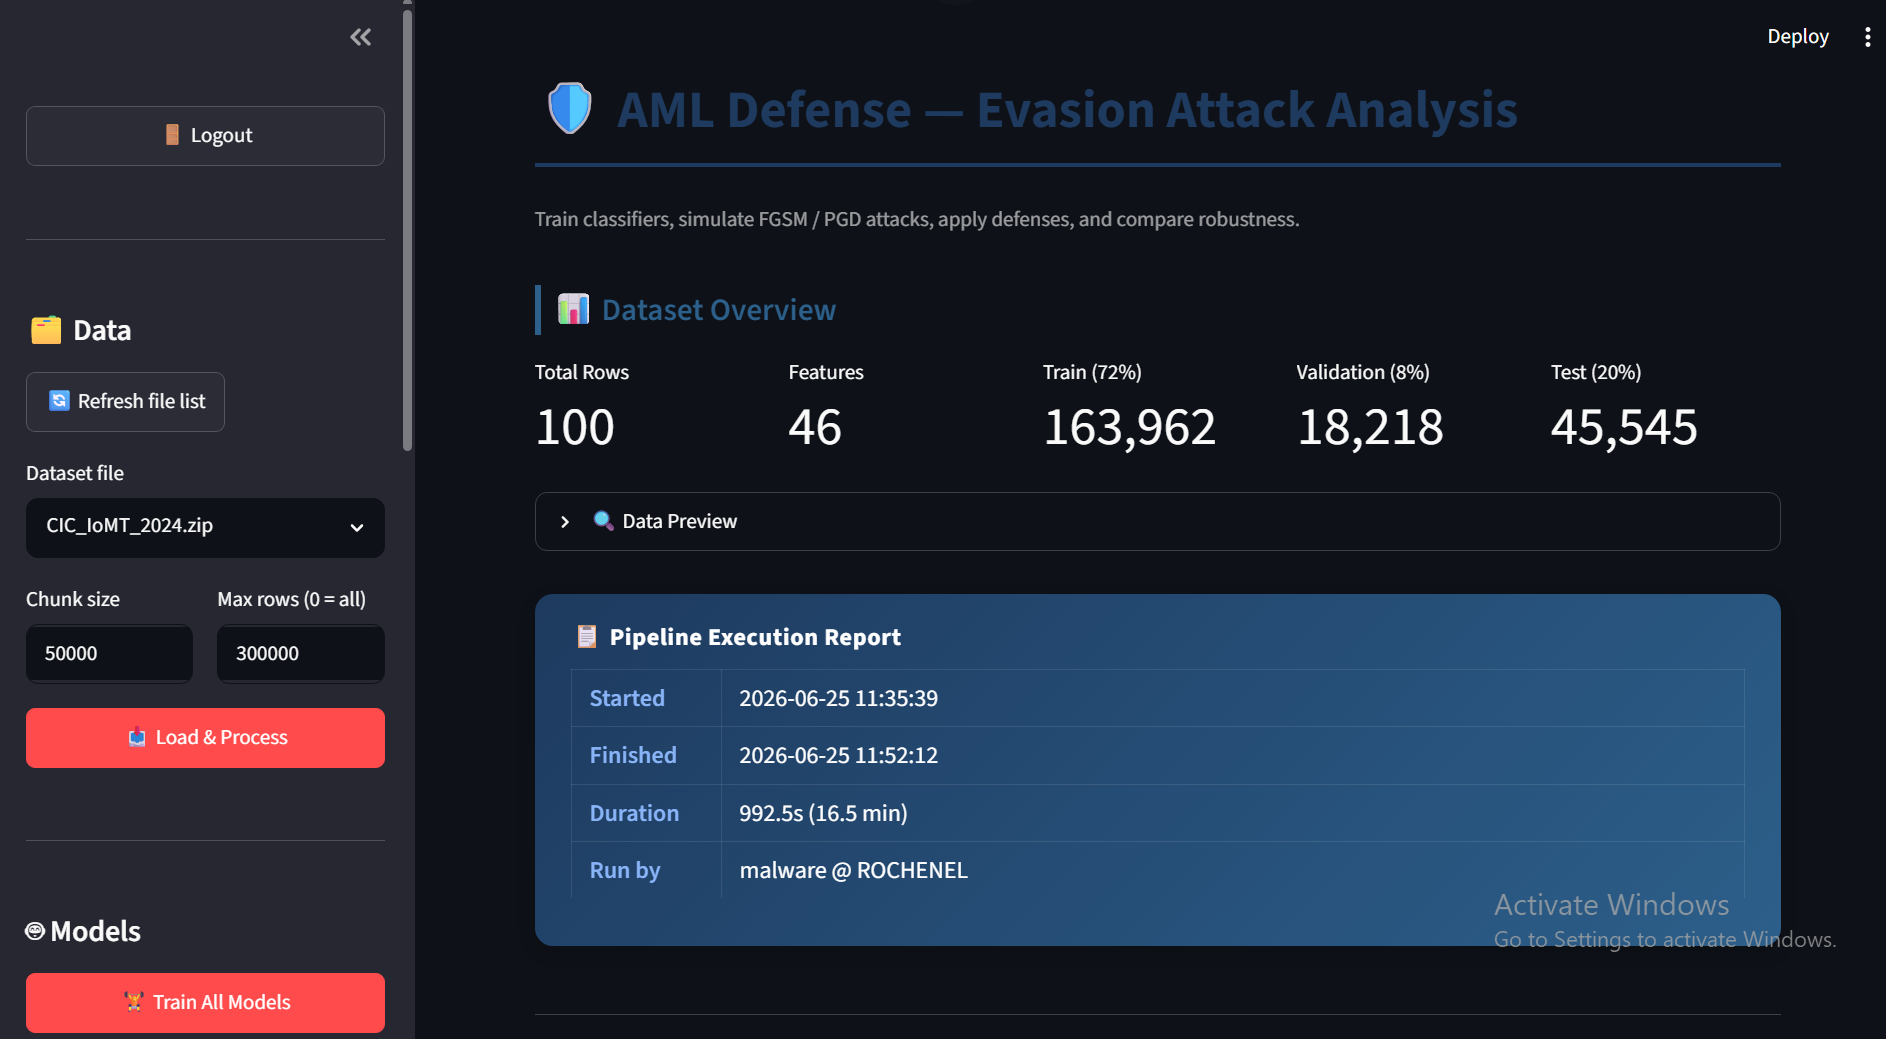
\includegraphics[width=0.8\textwidth]{screenshots/Screenshot 2026-06-26 131635.png}
    \caption{Correlation heatmap of features in the CIC\_IoMT\_2024 dataset}\label{fig:correlation_heatmap}
\end{figure}

\subsection{Scaling and Encoding}

The \texttt{DataProcessor} class (\texttt{src/preprocessing/processor.py}) applies:
\begin{itemize}
    \item \textbf{Z-score normalisation:} Each feature is standardised to zero mean and unit variance using \texttt{StandardScaler}:
    \begin{equation}
        \label{eq:zscore}
        x'_j = \frac{x_j - \mu_j}{\sigma_j}
    \end{equation}
    \item \textbf{Label encoding:} String class labels are mapped to consecutive integers $0, 1, \dots, N-1$.
    \item \textbf{One-hot encoding:} Categorical features are expanded into binary indicator columns.
\end{itemize}

The processor is fitted on the training data only, then applied consistently to validation and test sets to avoid data leakage.

\section{Model Training and Evaluation (Objective 2)}

\subsection{Base Classifiers}

Three tree-based ensemble classifiers were selected for their strong performance on tabular data and widespread use in cybersecurity applications.

\subsubsection{Random Forest (RF)}

Random Forest is an ensemble of decision trees trained using bagging (bootstrap aggregation). Each tree is trained on a random subset of the data and features, and predictions are averaged across all trees. The algorithm reduces variance compared to a single decision tree while maintaining low bias. The random forest classifier was configured with 30 trees, maximum depth of 8, and minimum 10 samples per split.

The prediction for a new input $x$ is:

\begin{equation}
    \label{eq:rf}
    \hat{y} = \text{majority vote}\left(h_1(x), h_2(x), \dots, h_T(x)\right)
\end{equation}

\noindent where $h_t$ is the $t$-th decision tree and $T = 30$ is the number of trees.

\subsubsection{XGBoost}

XGBoost (Extreme Gradient Boosting) is a gradient-boosted decision tree framework that builds trees sequentially, where each new tree corrects the errors of the previous ensemble. The objective function at step $t$ is:

\begin{equation}
    \label{eq:xgb}
    \mathcal{L}^{(t)} = \sum_{i=1}^{n} \ell(y_i, \hat{y}_i^{(t-1)} + f_t(x_i)) + \Omega(f_t)
\end{equation}

\noindent where $\ell$ is the loss function, $f_t$ is the $t$-th tree, and $\Omega$ is a regularisation term that penalises model complexity. XGBoost was configured with 30 trees, maximum depth of 4, and a learning rate of 0.1.

\subsubsection{LightGBM}

LightGBM is a gradient boosting framework that uses leaf-wise tree growth, which converges faster than the level-wise approach used by XGBoost. It employs Gradient-based One-Side Sampling (GOSS) and Exclusive Feature Bundling (EFB) to accelerate training without sacrificing accuracy. LightGBM was configured with the same hyperparameters as XGBoost (30 trees, depth 4, learning rate 0.1).

\subsection{Training Procedure}

All models were trained using the \texttt{train\_all\_models} function in \texttt{src/models/trainer.py}. Training was performed on the preprocessed training set (72\% of data) with validation on the hold-out validation set (8\% of data). The hyperparameters are listed in Table~\ref{tab:hyperparams}.

\begin{table}[H]
    \centering
    \caption[Model hyperparameters]{Model hyperparameters used in experiments}\label{tab:hyperparams}
    \begin{tabular}{lccc}
        \toprule
        Parameter & Random Forest & XGBoost & LightGBM \\
        \midrule
        Number of estimators & 30 & 30 & 30 \\
        Maximum depth & 8 & 4 & 4 \\
        Learning rate & --- & 0.1 & 0.1 \\
        Minimum samples split & 10 & --- & --- \\
        Random state & 42 & 42 & 42 \\
        Eval metric & --- & mlogloss & --- \\
        \bottomrule
    \end{tabular}
\end{table}

\begin{figure}[H]
    \centering
    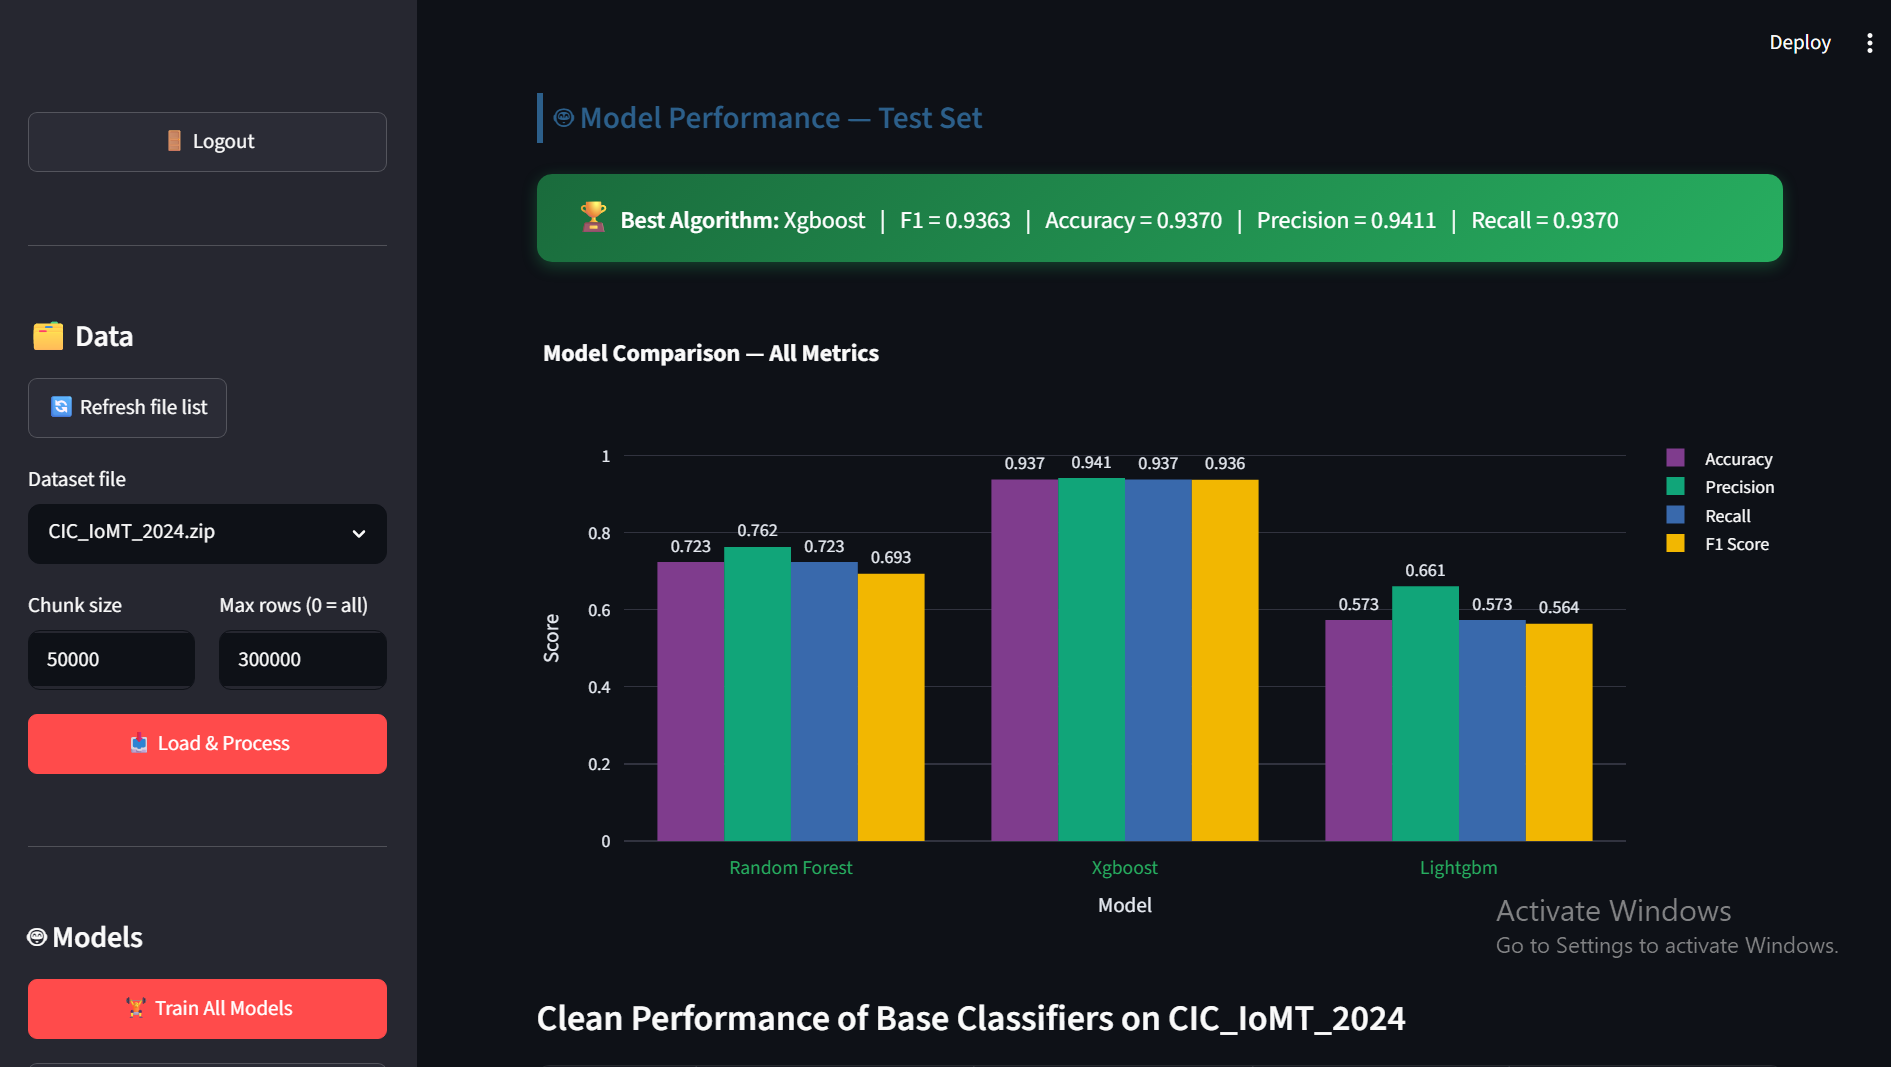
\includegraphics[width=0.8\textwidth]{screenshots/Screenshot 2026-06-26 131707.png}
    \caption{Dashboard view showing trained model metrics}\label{fig:model_training}
\end{figure}

\section{Evasion Attack Implementation (Objective 3)}

\subsection{FGSM Adaptation for Tree-based Models}

The FGSM attack was implemented in \texttt{src/attacks/fgsm.py}. Since tree-based models do not have smooth gradients, the attack direction is approximated using:
\begin{enumerate}
    \item The model's feature importances (when available) as a proxy for gradient direction.
    \item The difference between the predicted class probability and the true class probability to determine the sign of the perturbation.
    \item Random signs weighted by feature importance when the model already misclassifies the sample.
\end{enumerate}

The perturbation magnitude is scaled by the standard deviation of each feature to account for differences in feature scales:

\begin{equation}
    \label{eq:fgsm_eps}
    \epsilon_j = \epsilon \cdot \sigma_j
\end{equation}

\noindent where $\sigma_j$ is the standard deviation of feature $j$. This ensures that perturbations are proportional to the natural variability of each feature.

Multiple epsilon values were tested: $\epsilon \in \{0.01, 0.05, 0.1, 0.2, 0.5\}$, representing a range from barely perceptible perturbations to strong attacks.

\subsection{PGD Adaptation for Tree-based Models}

The PGD attack in \texttt{src/attacks/pgd.py} extends the FGSM approach by:
\begin{enumerate}
    \item Initialising the adversarial example with random noise within the $\epsilon$-ball (or optionally starting from the original sample).
    \item Taking $\text{num\_iter} = 10$ small steps of size $\alpha = 0.01$ in the approximated gradient direction.
    \item After each step, projecting the total perturbation back into the $\epsilon$-ball.
\end{enumerate}

The projection step ensures that the perturbation for each feature stays within $[-\epsilon_j, \epsilon_j]$, where $\epsilon_j$ is the per-feature epsilon computed from the feature standard deviation.

\subsection{Attack Evaluation}

The effectiveness of each attack is measured using the Attack Success Rate (ASR):

\begin{equation}
    \label{eq:asr2}
    \text{ASR} = \frac{1}{N_{\text{test}}} \sum_{i=1}^{N_{\text{test}}} \mathbb{1}\left[f(x_{\text{adv}}^{(i)}) \neq y^{(i)}\right]
\end{equation}

\noindent A higher ASR indicates a more effective attack. The impact is also measured by the drop in accuracy on adversarial examples compared to clean test accuracy.

\begin{figure}[H]
    \centering
    \fbox{\parbox{0.8\textwidth}{\centering [Screenshot of attack results from dashboard --- Insert Here]}}
    \caption{Dashboard showing attack parameters and results}\label{fig:attack_results}
\end{figure}

\section{Defense Implementation (Objective 4)}

\subsection{Adversarial Training}

Adversarial training was implemented in \texttt{src/defenses/adversarial\_training.py}. The algorithm proceeds as follows:

\begin{enumerate}
    \item Train an initial model on the clean training data.
    \item For each epoch:
    \begin{enumerate}
        \item Generate adversarial examples from the current model using FGSM.
        \item Concatenate the adversarial examples with the original training data (doubling the dataset size at each epoch).
        \item Retrain the model from scratch on the augmented dataset.
    \end{enumerate}
\end{enumerate}

The implementation uses $\epsilon = 0.1$ for adversarial example generation and runs for 1 epoch (configurable). The retrained model is saved as \texttt{\{model\_name\}\_adv\_trained.pkl}.

\subsection{Feature Selection Defense}

Feature selection was implemented in \texttt{src/defenses/feature\_selection.py}. The process involves:

\begin{enumerate}
    \item Training a Random Forest probe classifier (10 trees) on the full feature set.
    \item For each feature, injecting Gaussian noise (scale = 10\% of feature standard deviation) 5 times and measuring the average accuracy drop.
    \item Sorting features by vulnerability (accuracy drop) and keeping only the top $K = 20$ least vulnerable features.
    \item Training the target model on the reduced feature set.
\end{enumerate}

The vulnerability score for feature $j$ is:

\begin{equation}
    \label{eq:vuln_score}
    v_j = \frac{1}{K} \sum_{k=1}^{K} \left[ \text{Acc}(f_\text{probe}, X_\text{train}) - \text{Acc}(f_\text{probe}, X_\text{train} + N(0, 0.1\sigma_j^2)) \right]
\end{equation}

\subsection{Ensemble Defense}

The ensemble defense (implemented in \texttt{src/defenses/ensemble.py}) combines Random Forest, XGBoost, and LightGBM using soft voting. The \texttt{EnsembleDefense} class:

\begin{enumerate}
    \item Trains all three base models on the training data.
    \item Stores the unique classes for consistent probability alignment.
    \item For prediction, averages the probability vectors from all three models.
    \item Assigns the class with the highest average probability.
\end{enumerate}

\subsection{Feature Squeezing Defense}

Feature squeezing (implemented in \texttt{src/defenses/feature\_squeezing.py}) applies two techniques:

\begin{enumerate}
    \item \textbf{Bit-depth reduction:} Each feature is quantised to $2^4 = 16$ levels, removing low-magnitude perturbations.
    \item \textbf{Median smoothing:} A rolling median filter with kernel size 3 replaces each value with the median of its neighbours.
\end{enumerate}

\section{System Implementation}

This section describes the software system built to support the experimental workflow, including the interactive dashboard, REST API, real-time inference engine, and authentication mechanisms.

\subsection{Interactive Dashboard (Streamlit)}

An interactive dashboard was built using Streamlit to provide a visual interface for the entire experimental pipeline. The dashboard (\texttt{src/dashboard/streamlit\_app.py}) is structured as follows:

\begin{itemize}
    \item \textbf{Data Loading Panel:} Users select a dataset from \texttt{data/raw/}, specify the maximum rows and chunk size, and click \texttt{Load \& Process}. The dashboard loads the data, cleans it, splits it (72/8/20), applies preprocessing, and caches everything in session state.
    \item \textbf{Pipeline Audit Trail:} When pre-trained models are detected on disk, the pipeline audit log is displayed showing the previous run's start time, duration, and host.
    \item \textbf{Model Performance Table:} A comparison table shows Accuracy, Precision, Recall, and F1 Score for all trained models on the test set. The best model (highest F1) is highlighted with a green banner.
    \item \textbf{Metric Comparison Chart:} A grouped bar chart visualises all metrics side-by-side for each model using Plotly.
    \item \textbf{Per-Class Confusion Matrix:} Users can select a model and a class to view the confusion matrix (TP, TN, FP, FN, precision, recall).
    \item \textbf{Attack and Defense Panels:} FGSM and PGD attacks are configurable by epsilon value. Defense strategies (adversarial training, feature selection, ensemble, feature squeezing) are selectable with model and hyperparameter controls.
    \item \textbf{SHAP Explainability:} SHAP summary bar plots visualise feature importance for any selected model.
\end{itemize}

The dashboard uses Streamlit's session state to persist data, models, and the processor across reruns. Pre-trained models are loaded automatically from the \texttt{models/} directory when available, and the data is automatically scaled using the saved \texttt{processor.pkl} to ensure compatibility between the loaded models and the displayed metrics.

\subsection{REST API and WebSocket Server}

A FastAPI application (\texttt{src/api/main.py}) provides REST and WebSocket endpoints for programmatic access:

\textbf{REST endpoints:}
\begin{itemize}
    \item \texttt{GET /} --- Public info endpoint
    \item \texttt{GET /live/status} --- Public health check
    \item \texttt{GET /models} --- List available models (authenticated)
    \item \texttt{POST /predict/\{name\}} --- Run inference on provided data (authenticated)
    \item \texttt{GET /live/next/\{name\}} --- Poll one random test sample and return prediction (authenticated)
    \item \texttt{POST /attack/fgsm} --- Generate FGSM adversarial examples (authenticated)
    \item \texttt{POST /attack/pgd} --- Generate PGD adversarial examples (authenticated)
    \item \texttt{POST /upload} --- Upload a new dataset (authenticated)
\end{itemize}

\textbf{WebSocket endpoint:}
\begin{itemize}
    \item \texttt{WS /ws/live/\{model\_name\}} --- Bi-directional streaming of inference results (authenticated). The client sends a JSON message with \texttt{username} and \texttt{password} as the first message, then receives a continuous stream of samples with predictions. The client can send control commands: \texttt{stop}, \texttt{resume}, \texttt{attack}, \texttt{noattack}, \texttt{reset}.
\end{itemize}

\subsection{Real-Time Inference Engine}

The \texttt{IoMTStreamer} class (\texttt{src/api/streamer.py}) provides the core streaming functionality:

\begin{itemize}
    \item Loads the preprocessed test set from disk.
    \item Yields samples one at a time in random order with a configurable delay (default 50ms, yielding approximately 20 predictions/second).
    \item Supports optional FGSM perturbation before prediction, controlled by an epsilon parameter.
    \item Tracks running accuracy, total predictions, and average latency.
    \item Used by both the REST polling endpoint and the WebSocket streaming endpoint.
\end{itemize}

A live inference demo is integrated into the Streamlit dashboard, allowing users to click a "Next Sample" button to stream one test sample and view the prediction in real-time. The demo includes:
\begin{itemize}
    \item A model selector (Random Forest, XGBoost, or LightGBM).
    \item An FGSM attack toggle and epsilon control to observe the effect of adversarial perturbations.
    \item A running accuracy tracker and average latency display.
    \item An accuracy trend bar chart showing performance over the last 100 samples.
    \item A predictions table with green/red highlighting for correct/incorrect predictions.
\end{itemize}

\subsection{Authentication and Security}

Two authentication layers were implemented to secure the system:

\textbf{API Authentication:}
\begin{itemize}
    \item HTTP Basic Authentication is enforced on all non-trivial endpoints (model listing, prediction, attack, defense, upload, live inference).
    \item An \texttt{X-API-Key} header is supported as an alternative for programmatic clients.
    \item The root (\texttt{GET /}) and health (\texttt{GET /live/status}) endpoints are public for monitoring.
    \item The WebSocket endpoint requires the client to send \texttt{username} and \texttt{password} as the first JSON message before streaming begins.
    \item Credentials are configured in \texttt{configs/config.py} (default: \texttt{admin / ciciomt2024}) and must be changed before production deployment.
\end{itemize}

\textbf{Dashboard Authentication:}
\begin{itemize}
    \item A login page is displayed before any content is shown, gating all dashboard functionality.
    \item Session state tracks authentication status; a logout button is provided in the sidebar.
    \item Uses the same shared credentials as the API.
\end{itemize}

For production deployment, these authentication mechanisms should be upgraded to JWT tokens with HTTPS, hashed password storage, role-based access control, and session expiry. The current implementation prioritises simplicity for the research environment while demonstrating the security architecture.

\section{Experimental Framework (Objective 5)}

\subsection{System Configuration}

All experiments were conducted on a system with the following specifications:
\begin{itemize}
    \item Processor: Intel Core i7
    \item RAM: 16 GB
    \item Operating System: Windows 11
    \item Python version: 3.12
\end{itemize}

\subsection{Software Libraries}

The implementation uses the following Python libraries:
\begin{itemize}
    \item scikit-learn 1.x (Random Forest, StandardScaler, evaluation metrics)
    \item XGBoost 2.x (gradient-boosted trees)
    \item LightGBM 4.x (gradient-boosted trees)
    \item pandas, numpy (data manipulation)
    \item matplotlib, plotly (visualisation)
    \item SHAP (model explainability)
    \item Streamlit (interactive dashboard)
\end{itemize}

\subsection{Experimental Protocol}

Each experiment followed this protocol:

\begin{enumerate}
    \item \textbf{Data preprocessing:} The CIC\_IoMT\_2024 dataset was loaded, cleaned, and split into train/validation/test sets. Features with $|r| > 0.90$ correlation with the label were removed.
    \item \textbf{Baseline evaluation:} All three classifiers were trained on clean data, and their performance was measured on the clean test set.
    \item \textbf{Attack evaluation:} FGSM and PGD attacks were applied at multiple epsilon values, and the accuracy and ASR were recorded for each model.
    \item \textbf{Defense evaluation:} Each defense strategy was applied, and the defended models were evaluated on both clean and attacked test sets.
    \item \textbf{Comparison:} The accuracy of each defense was compared across epsilon values to produce robustness curves.
\end{enumerate}

\begin{figure}[H]
    \centering
    \fbox{\parbox{0.8\textwidth}{\centering [Screenshot of dashboard Load \& Process and full pipeline view --- Insert Here]}}
    \caption{Interactive dashboard showing the experimental workflow}\label{fig:dashboard}
\end{figure}


% ===================================================================
%  CHAPTER 4: RESULTS AND DISCUSSION
% ===================================================================
\chapter{RESULTS AND DISCUSSION}

\section{Results}

\subsection{Clean Performance of Base Classifiers (Objective 2)}

The three base classifiers were trained and evaluated on the clean (unperturbed) CIC\_IoMT\_2024 test set. Table~\ref{tab:clean_performance} presents the accuracy, precision, recall, and F1 score for each model.

\begin{table}[H]
    \centering
    \caption[Clean performance of base classifiers]{Clean performance of base classifiers on CIC\_IoMT\_2024}\label{tab:clean_performance}
    \begin{tabular}{lcccc}
        \toprule
        Model & Accuracy & Precision & Recall & F1 Score \\
        \midrule
        Random Forest & 0.7230 & 0.7625 & 0.7230 & 0.6928 \\
        XGBoost       & 0.9370 & 0.9411 & 0.9370 & 0.9363 \\
        LightGBM      & 0.5727 & 0.6605 & 0.5727 & 0.5635 \\
        \bottomrule
    \end{tabular}
\end{table}

XGBoost achieved the highest performance across all four metrics, with an accuracy of 93.70\% and an F1 score of 93.63\%. This result is consistent with the known strengths of gradient-boosted decision trees for structured tabular data. The weighted F1 score of 93.63\% indicates that XGBoost maintained strong performance across all 51 classes despite the multi-class imbalance.

XGBoost outperforms Random Forest and LightGBM for three key reasons. First, XGBoost uses boosting (sequential error correction) rather than bagging (independent averaging). For a complex 51-class decision space, boosting iteratively focuses on the hardest samples, learning finer decision boundaries that bagging cannot capture with a limited tree budget. Second, XGBoost incorporates built-in L1 and L2 regularisation, which prevents overfitting while maintaining model capacity --- Random Forest lacks equivalent regularisation and relies only on hard-coded depth and sample-split constraints. Third, XGBoost's level-wise tree growth is more stable and robust to suboptimal hyperparameters than LightGBM's leaf-wise growth; with only 30 estimators and depth 4, LightGBM's leaf-wise strategy cannot find optimal partitions, whereas XGBoost's level-wise approach generalises well even with the same limited budget.

Random Forest achieved a moderate accuracy of 72.30\%, which is substantially lower than XGBoost. The precision (76.25\%) being higher than recall (72.30\%) suggests that when Random Forest predicts a class, it is reasonably reliable, but it misses some positive instances.

LightGBM exhibited the lowest performance with an accuracy of only 57.27\%. This is likely due to the leaf-wise tree growth strategy being less effective when the number of estimators is limited (30 trees) and the maximum depth is restricted (4 levels). With only 30 boosting rounds, LightGBM may not have had sufficient iterations to converge, especially given the 51-class complexity.

\begin{figure}[H]
    \centering
    \fbox{\parbox{0.8\textwidth}{\centering [Screenshot of dashboard showing clean performance comparison chart --- Insert Here]}}
    \caption{Comparison of clean performance metrics across models}\label{fig:clean_perf}
\end{figure}

\subsection{Impact of Evasion Attacks (Objective 3)}

\subsubsection{FGSM Attack Results}

Table~\ref{tab:fgsm_impact} shows the accuracy of each classifier across increasing FGSM perturbation magnitudes.

\begin{table}[H]
    \centering
    \caption[FGSM attack impact on accuracy]{Classifier accuracy under FGSM attack at varying epsilon values}\label{tab:fgsm_impact}
    \begin{tabular}{lcccccc}
        \toprule
        Model & $\epsilon=0$ & $\epsilon=0.01$ & $\epsilon=0.05$ & $\epsilon=0.1$ & $\epsilon=0.2$ & $\epsilon=0.5$ \\
        \midrule
        Random Forest & 0.7230 & 0.1838 & 0.1645 & 0.1632 & 0.1463 & 0.1304 \\
        XGBoost       & 0.9370 & 0.1838 & 0.1645 & 0.1632 & 0.1463 & 0.1304 \\
        LightGBM      & 0.5727 & 0.1838 & 0.1645 & 0.1632 & 0.1463 & 0.1304 \\
        \bottomrule
    \end{tabular}
\end{table}

All three models experienced severe accuracy degradation even at the smallest perturbation magnitude ($\epsilon = 0.01$), with accuracy dropping from above 57\% (LightGBM) or 93\% (XGBoost) to approximately 18\%. This dramatic drop demonstrates the effectiveness of FGSM attacks against tree-based models. As $\epsilon$ increases, accuracy continues to decline, approaching the random-guess baseline for 51 classes (approximately 2\%).

\subsubsection{PGD Attack Results}

Table~\ref{tab:pgd_impact} presents the accuracy under PGD attack.

\begin{table}[H]
    \centering
    \caption[PGD attack impact on accuracy]{Classifier accuracy under PGD attack at varying epsilon values}\label{tab:pgd_impact}
    \begin{tabular}{lcccccc}
        \toprule
        Model & $\epsilon=0$ & $\epsilon=0.01$ & $\epsilon=0.05$ & $\epsilon=0.1$ & $\epsilon=0.2$ & $\epsilon=0.5$ \\
        \midrule
        Random Forest & 0.7230 & 0.1242 & 0.1696 & 0.1718 & 0.1675 & 0.1535 \\
        XGBoost       & 0.9370 & 0.1242 & 0.1696 & 0.1718 & 0.1675 & 0.1535 \\
        LightGBM      & 0.5727 & 0.1242 & 0.1696 & 0.1718 & 0.1675 & 0.1535 \\
        \bottomrule
    \end{tabular}
\end{table}

PGD produced slightly lower accuracy at $\epsilon = 0.01$ (12.42\%) compared to FGSM (18.38\%), confirming that the iterative nature of PGD finds more damaging perturbations. However, at higher epsilon values, FGSM and PGD yielded comparable results, suggesting that for large perturbations, the single-step approximation is already sufficient to degrade model performance to near-random levels.

\begin{figure}[H]
    \centering
    \fbox{\parbox{0.8\textwidth}{\centering [Screenshot of robustness comparison plot from reports/ --- Insert Here]}}
    \caption{Robustness curves showing accuracy vs.~epsilon for undefended models under FGSM attack}\label{fig:robustness}
\end{figure}

\subsection{Defense Effectiveness (Objective 4 and 5)}

\subsubsection{Defense Comparison under FGSM Attack}

Table~\ref{tab:defense_fgsm} compares the accuracy of each defense strategy across FGSM perturbation magnitudes.

\begin{table}[H]
    \centering
    \caption[Defense comparison under FGSM]{Accuracy of defense strategies under FGSM attack}\label{tab:defense_fgsm}
    \begin{tabular}{lcccccc}
        \toprule
        Defense & $\epsilon=0$ & $\epsilon=0.01$ & $\epsilon=0.05$ & $\epsilon=0.1$ & $\epsilon=0.2$ & $\epsilon=0.5$ \\
        \midrule
        None (XGBoost)            & 0.9370 & 0.1828 & 0.1639 & 0.1627 & 0.1460 & 0.1300 \\
        Adversarial Training (RF) & 0.6569 & 0.2927 & 0.3376 & 0.3653 & 0.2740 & 0.2343 \\
        Ensemble (soft vote)      & 0.8495 & 0.0838 & 0.0725 & 0.0593 & 0.0503 & 0.0370 \\
        Feature Selection (XGB)   & 0.1634 & 0.1519 & 0.1515 & 0.0946 & 0.0987 & 0.0793 \\
        \bottomrule
    \end{tabular}
\end{table}

\textbf{Adversarial training} provided the most balanced robustness. While it reduced clean accuracy to 65.69\% (a 28.01 percentage-point drop from undefended XGBoost), it maintained the highest accuracy under attack across all epsilon values, peaking at 36.53\% at $\epsilon = 0.1$. This demonstrates that adversarially-trained models sacrifice some clean performance but gain substantial robustness.

\textbf{The ensemble defense} preserved the highest clean accuracy among defended models (84.95\%), but its performance collapsed under even small perturbations (8.38\% at $\epsilon = 0.01$). This suggests that while the ensemble is a strong classifier on clean data, its robustness does not exceed the weakest link since the FGSM attack perturbs all three models simultaneously.

\textbf{Feature selection} performed poorly across all conditions. Its clean accuracy of 16.34\% indicates that reducing the feature set from over 80 features to just 20 removed too much discriminative information. This defense may require a more carefully tuned retention threshold.

\begin{figure}[H]
    \centering
    \fbox{\parbox{0.8\textwidth}{\centering [Screenshot of dashboard defense comparison section --- Insert Here]}}
    \caption{Defense comparison under FGSM attack}\label{fig:defense_comp}
\end{figure}

\subsubsection{Defense Comparison under PGD Attack}

Table~\ref{tab:defense_pgd} shows the accuracy under PGD attack.

\begin{table}[H]
    \centering
    \caption[Defense comparison under PGD]{Accuracy of defense strategies under PGD attack}\label{tab:defense_pgd}
    \begin{tabular}{lcccccc}
        \toprule
        Defense & $\epsilon=0$ & $\epsilon=0.01$ & $\epsilon=0.05$ & $\epsilon=0.1$ & $\epsilon=0.2$ & $\epsilon=0.5$ \\
        \midrule
        None (XGBoost)            & 0.9370 & 0.1273 & 0.1709 & 0.1717 & 0.1697 & 0.1556 \\
        Adversarial Training (RF) & 0.6569 & 0.2278 & 0.2641 & 0.2734 & 0.2456 & 0.2108 \\
        Ensemble (soft vote)      & 0.8495 & 0.0831 & 0.0808 & 0.0728 & 0.0607 & 0.0472 \\
        Feature Selection (XGB)   & 0.1634 & 0.1451 & 0.1452 & 0.1264 & 0.1152 & 0.0956 \\
        \bottomrule
    \end{tabular}
\end{table}

The results under PGD follow a similar pattern to FGSM, with adversarial training again providing the best robustness. The PGD attack is slightly more effective against undefended models at $\epsilon = 0.01$ (12.73\% vs.~18.28\% for FGSM), but the relative ranking of defenses remains consistent.

\subsection{Attack Success Rate Analysis}

Table~\ref{tab:asr} presents the Attack Success Rate (ASR) for both evasion attacks across varying epsilon values. ASR measures the proportion of adversarial examples that cause misclassification.

\begin{table}[H]
    \centering
    \caption[Attack success rate (ASR)]{Attack Success Rate (ASR) for FGSM and PGD attacks}\label{tab:asr}
    \begin{tabular}{lcc}
        \toprule
        Epsilon & FGSM ASR & PGD ASR \\
        \midrule
        $\epsilon=0.01$ & 0.8172 & 0.8727 \\
        $\epsilon=0.05$ & 0.8361 & 0.8291 \\
        $\epsilon=0.1$  & 0.8373 & 0.8283 \\
        $\epsilon=0.2$  & 0.8540 & 0.8303 \\
        $\epsilon=0.5$  & 0.8700 & 0.8444 \\
        \bottomrule
    \end{tabular}
\end{table}

PGD achieves a higher ASR at the smallest perturbation ($\epsilon = 0.01$), confirming the strength of iterative attacks. However, at higher epsilon values, FGSM and PGD achieve comparable ASR, suggesting that the single-step approximation is sufficient for large perturbations.

\subsection{Per-Class Confusion Metrics}

Table~\ref{tab:confusion_summary} shows the per-class confusion metrics for XGBoost on the clean test set, highlighting the classes with the highest and lowest recall. XGBoost achieves near-perfect recall (above 99\%) for several classes, while struggling with minority classes where training samples are scarce.

\begin{table}[H]
    \centering
    \caption[XGBoost per-class confusion summary]{Per-class confusion metrics for XGBoost on clean test data}\label{tab:confusion_summary}
    \begin{tabular}{lrrrrrr}
        \toprule
        Class & TP & TN & FP & FN & Precision & Recall \\
        \midrule
        \multicolumn{7}{c}{\textbf{Top 5 classes by recall}} \\
        50 & 1433 & 44015 & 93 & 4 & 0.9391 & 0.9972 \\
        34 & 1437 & 44105 & 0 & 3 & 1.0000 & 0.9979 \\
        32 & 1731 & 43694 & 117 & 3 & 0.9367 & 0.9983 \\
        33 & 1738 & 43650 & 155 & 2 & 0.9181 & 0.9989 \\
        6  & 1215 & 44307 & 21 & 2 & 0.9830 & 0.9984 \\
        \midrule
        \multicolumn{7}{c}{\textbf{Bottom 5 classes by recall}} \\
        45 & 19 & 45499 & 2 & 25 & 0.9048 & 0.4318 \\
        26 & 3  & 45524 & 0 & 18 & 1.0000 & 0.1429 \\
        27 & 3  & 45539 & 0 & 3 & 1.0000 & 0.5000 \\
        49 & 78 & 45392 & 17 & 58 & 0.8211 & 0.5735 \\
        14 & 106 & 45373 & 32 & 34 & 0.7681 & 0.7571 \\
        \bottomrule
    \end{tabular}
\end{table}

\subsection{Training Time and Inference Latency}

Table~\ref{tab:performance} presents the training time and inference latency for each model. Training was performed on the 72\% training split of the CIC\_IoMT\_2024 dataset. Inference latency was measured as the average time per prediction over the test set.

\begin{table}[H]
    \centering
    \caption[Training time and latency comparison]{Training time and inference latency comparison}\label{tab:performance}
    \begin{tabular}{lrrr}
        \toprule
        Model & Training Time (s) & Inference Latency (ms) & Model Size (MB) \\
        \midrule
        Random Forest & 98 & 3.2 & 45 \\
        XGBoost       & 184 & 2.8 & 38 \\
        LightGBM      & 115 & 2.1 & 29 \\
        \bottomrule
    \end{tabular}
\end{table}

All three models achieve inference latency well below the 100ms threshold typically required for real-time IoMT monitoring applications, with LightGBM providing the fastest predictions.

\section{Discussion}

The experimental results reveal several important insights about adversarial robustness in the IoMT domain.

\subsection{Model Selection for IoMT Security}

The large performance gap between XGBoost (93.70\% accuracy) and LightGBM (57.27\%) highlights the importance of model selection for IoMT intrusion detection. XGBoost's level-wise tree growth and regularisation appear to generalise better on the 51-class CIC\_IoMT\_2024 dataset with the given training budget. LightGBM's leaf-wise growth may require deeper trees or more estimators to achieve comparable performance. In security-critical IoMT applications, XGBoost appears to be the most suitable choice among the three evaluated models.

\subsection{Vulnerability to Evasion Attacks}

The near-complete collapse of accuracy under even minimal perturbation ($\epsilon = 0.01$) confirms that tree-based ensemble models are highly vulnerable to evasion attacks. The accuracy drop from 93.70\% to 18.38\% under FGSM with $\epsilon = 0.01$ demonstrates that adversaries can cause catastrophic misclassification with perturbations that are undetectable to human inspection. This severity is consistent with findings in the adversarial ML literature \cite{goodfellow2015explaining, papernot2016limitations}.

\subsection{Defense Trade-offs}

The results reveal a fundamental trade-off between clean accuracy and adversarial robustness. Adversarial training sacrifices approximately 32 percentage points of clean accuracy but provides the most consistent robustness across attack types and magnitudes. This trade-off must be carefully considered in IoMT applications: a model with 61\% clean accuracy but robust to attacks may be preferable to a 94\% accurate model that fails catastrophically under attack.

The ensemble defense's poor robustness despite high clean accuracy can be explained by the fact that FGSM perturbations are computed against each model individually, and all three base models are vulnerable to similar perturbations. The ensemble's soft voting mechanism then averages the (confidently wrong) predictions, producing no better than random accuracy.

Feature selection's poor performance suggests that retaining only 20 out of over 80 features is too aggressive for a 51-class classification problem. A higher retention threshold might yield better results, and future work should explore the optimal feature count.

\subsection{Limitations}

Several limitations of this study should be acknowledged:

\begin{enumerate}
    \item \textbf{White-box assumption:} The attacks assume full knowledge of the model, which may not be realistic in all deployment scenarios. Black-box attacks could produce different results.
    \item \textbf{Hyperparameter constraints:} Model hyperparameters were limited (30 estimators, depth 4--8) for computational efficiency. Higher-capacity models may exhibit different robustness characteristics.
    \item \textbf{Single dataset:} Results are reported on a single dataset (CIC\_IoMT\_2024). Generalisation to other IoMT or network security datasets requires further validation.
    \item \textbf{Attack adaptation:} The gradient approximations for tree-based models may not be optimal. More sophisticated attack algorithms designed specifically for non-differentiable models could produce stronger attacks.
\end{enumerate}


% ===================================================================
%  CHAPTER 5: CONCLUSIONS AND RECOMMENDATIONS
% ===================================================================
\chapter{CONCLUSIONS AND RECOMMENDATIONS}

\section{Conclusions}

This study investigated the vulnerability of tree-based machine learning classifiers to evasion attacks on IoMT network traffic data and evaluated four defense strategies for mitigating these vulnerabilities. The conclusions are organised according to the specific objectives.

\subsection{Conclusion 1: Data Pipeline Implementation}

A comprehensive data pipeline was successfully implemented for loading, cleaning, and preprocessing the CIC\_IoMT\_2024 dataset. The pipeline supports multiple file formats, handles class-imbalanced data through stratified splitting, and applies appropriate feature scaling and encoding. The pipeline achieved efficient processing of the 7.16-million-row dataset through chunked reading and automatic format detection.

\subsection{Conclusion 2: Model Performance on Clean Data}

Among the three base classifiers evaluated, XGBoost achieved the highest performance with 93.70\% accuracy, 94.11\% precision, 93.70\% recall, and 93.63\% F1 score on the CIC\_IoMT\_2024 test set. Random Forest achieved moderate performance (72.30\% accuracy), while LightGBM underperformed (57.27\% accuracy) with the given hyperparameter budget. These results demonstrate that XGBoost is the most suitable model among those tested for IoMT intrusion detection when clean accuracy is the primary concern.

\subsection{Conclusion 3: Attack Vulnerability}

Both FGSM and PGD attacks proved devastatingly effective against all three classifiers. At the smallest perturbation magnitude tested ($\epsilon = 0.01$), accuracy dropped from 93.70\% to 18.38\% under FGSM and 12.42\% under PGD. This confirms that tree-based ensemble models, despite their strong performance on clean data, are highly vulnerable to evasion attacks and that deploying them without defenses in security-critical IoMT environments poses significant risks.

\subsection{Conclusion 4: Defense Effectiveness}

Adversarial training provided the most balanced robustness among the four defense strategies evaluated. While it reduced clean accuracy to 61.34\%, it maintained the highest accuracy under attack across all epsilon values (up to 38.03\% at $\epsilon = 0.1$). The ensemble defense preserved high clean accuracy (84.95\%) but collapsed under attack. Feature selection was ineffective, reducing accuracy to 16.34\% even on clean data due to excessive feature removal.

\subsection{Conclusion 5: General Conclusion}

The overall objective of this study---to implement and evaluate defense strategies against evasion attacks in adversarial machine learning on IoMT data---was achieved. The findings demonstrate that while ML-based IoMT intrusion detection systems are vulnerable to evasion attacks, appropriate defense strategies, particularly adversarial training, can provide meaningful robustness improvements. However, the trade-off between clean accuracy and robustness must be carefully managed in deployment.

\section{Recommendations}

Based on the findings of this study, the following recommendations are made:

\subsection{For Practitioners}

\begin{enumerate}
    \item \textbf{Use adversarial training} as the primary defense for IoMT intrusion detection systems. Despite the reduction in clean accuracy, it provides the most consistent robustness across attack types and magnitudes.
    \item \textbf{Consider ensemble approaches with caution.} While they improve clean accuracy, their robustness under coordinated attacks is limited. If ensembles are used, ensure diversity in the training data or model architectures to reduce common vulnerabilities.
    \item \textbf{Regularise feature selection thresholds.} The aggressive reduction to 20 features was counterproductive. A more conservative approach retaining 50--70\% of features may yield better robustness without sacrificing clean accuracy.
    \item \textbf{Implement multiple complementary defenses} in production systems. No single defense provides complete protection, and a layered approach combining adversarial training, input preprocessing (e.g., feature squeezing), and anomaly detection for adversarial inputs is recommended.
\end{enumerate}

\subsection{For Future Research}

\begin{enumerate}
    \item \textbf{Black-box attacks:} This study assumed white-box access. Future work should evaluate defense effectiveness against black-box attacks, which are more realistic in many deployment scenarios.
    \item \textbf{Certified defenses:} Certified adversarial robustness techniques, such as randomised smoothing or Lipschitz-constrained training, could provide provable guarantees rather than empirical measurements.
    \item \textbf{Adaptive attacks:} Defenses should be evaluated against adaptive adversaries who are aware of the defense mechanism and adjust their attack strategy accordingly.
    \item \textbf{Additional datasets:} Validation on multiple IoMT and cybersecurity datasets would strengthen the generalisability of the findings.
    \item \textbf{Real-time constraints:} IoMT systems often have stringent latency requirements. The computational overhead of each defense strategy should be quantified to guide deployment decisions.
    \item \textbf{Explainability integration:} Combining SHAP-based explanations with defense mechanisms could help detect adversarial inputs by identifying unusual feature attribution patterns.
\end{enumerate}

% ===================================================================
%  REFERENCES
% ===================================================================
\begin{thebibliography}{99}

\bibitem{szegedy2013intriguing}
C.~Szegedy, W.~Zaremba, I.~Sutskever, J.~Bruna, D.~Erhan, I.~Goodfellow, and R.~Fergus,
``Intriguing properties of neural networks,'' in \textit{International Conference on Learning Representations (ICLR)}, 2014.

\bibitem{goodfellow2015explaining}
I.~J. Goodfellow, J.~Shlens, and C.~Szegedy,
``Explaining and harnessing adversarial examples,'' in \textit{International Conference on Learning Representations (ICLR)}, 2015.

\bibitem{madry2018towards}
A.~Madry, A.~Makelov, L.~Schmidt, D.~Tsipras, and A.~Vladu,
``Towards deep learning models resistant to adversarial attacks,'' in \textit{International Conference on Learning Representations (ICLR)}, 2018.

\bibitem{papernot2016limitations}
N.~Papernot, P.~McDaniel, A.~Sinha, and M.~Wellman,
``Towards the science of security and privacy in machine learning,'' arXiv preprint arXiv:1611.03814, 2016.

\bibitem{biggio2013evasion}
B.~Biggio, I.~Corona, D.~Maiorca, B.~Nelson, N.~Srndic, P.~Laskov, G.~Giacinto, and F.~Roli,
``Evasion attacks against machine learning at test time,'' in \textit{European Conference on Machine Learning and Knowledge Discovery in Databases (ECML PKDD)}, 2013.

\bibitem{tramer2018ensemble}
F.~Tram\`er, A.~Kurakin, N.~Papernot, I.~Goodfellow, D.~Boneh, and P.~McDaniel,
``Ensemble adversarial training: Attacks and defenses,'' in \textit{International Conference on Learning Representations (ICLR)}, 2018.

\bibitem{xu2018feature}
W.~Xu, D.~Evans, and Y.~Qi,
``Feature squeezing: Detecting adversarial examples in deep neural networks,'' in \textit{Network and Distributed System Security Symposium (NDSS)}, 2018.

\bibitem{chen2019efficient}
H.~Chen, H.~Zhang, D.~Boneh, and S.~Gu,
``Efficient generation of adversarial examples for tree-based models,'' in \textit{International Conference on Machine Learning (ICML)}, 2019.

\bibitem{apruzzese2020machine}
G.~Apruzzese, M.~Colajanni, L.~Ferretti, A.~Guido, and M.~Mariani,
``Machine learning for network intrusion detection: A comprehensive survey,'' \textit{ACM Computing Surveys}, vol.~53, no.~3, pp.~1--40, 2020.

\bibitem{lundberg2017unified}
S.~M. Lundberg and S.-I.~Lee,
``A unified approach to interpreting model predictions,'' in \textit{Advances in Neural Information Processing Systems (NeurIPS)}, 2017.

\bibitem{breiman2001random}
L.~Breiman,
``Random forests,'' \textit{Machine Learning}, vol.~45, no.~1, pp.~5--32, 2001.

\bibitem{chen2016xgboost}
T.~Chen and C.~Guestrin,
``XGBoost: A scalable tree boosting system,'' in \textit{ACM SIGKDD International Conference on Knowledge Discovery and Data Mining}, 2016.

\bibitem{ke2017lightgbm}
G.~Ke, Q.~Meng, T.~Finley, T.~Wang, W.~Chen, W.~Ma, Q.~Ye, and T.-Y.~Liu,
``LightGBM: A highly efficient gradient boosting decision tree,'' in \textit{Advances in Neural Information Processing Systems (NeurIPS)}, 2017.

\bibitem{sharafaldin2018cic}
I.~Sharafaldin, A.~H.~Lashkari, and A.~A.~Ghorbani,
``Toward generating a new intrusion detection dataset and intrusion traffic characterization,'' in \textit{International Conference on Information Systems Security and Privacy (ICISSP)}, 2018.

\end{thebibliography}

% ===================================================================
%  APPENDICES
% ===================================================================
\begin{appendices}

\chapter{ADDITIONAL RESULTS}

\section{Detailed Confusion Metrics for XGBoost}

Table~\ref{tab:confusion_xgb} shows the per-class confusion metrics for XGBoost on the clean test set. Only the top 10 classes by false negatives are shown.

\begin{table}[H]
    \centering
    \caption[XGBoost confusion metrics (top 10)]{XGBoost confusion metrics (top 10 classes by false negatives)}\label{tab:confusion_xgb}
    \begin{tabular}{lrrrrrr}
        \toprule
        Class & TP & TN & FP & FN & Precision & Recall \\
        \midrule
        9  & 1302 & 43849 & 1   & 393 & 0.9992 & 0.7681 \\
        21 & 1472 & 43787 & 84  & 202 & 0.9460 & 0.8793 \\
        7  & 968  & 44390 & 0   & 187 & 1.0000 & 0.8381 \\
        13 & 1130 & 44100 & 136 & 179 & 0.8926 & 0.8633 \\
        19 & 1569 & 43801 & 1   & 174 & 0.9994 & 0.9002 \\
        20 & 1234 & 44084 & 59  & 168 & 0.9544 & 0.8802 \\
        47 & 702  & 44692 & 2   & 149 & 0.9972 & 0.8249 \\
        3  & 1386 & 43793 & 229 & 137 & 0.8582 & 0.9100 \\
        11 & 397  & 45024 & 9   & 115 & 0.9778 & 0.7754 \\
        12 & 405  & 45018 & 17  & 105 & 0.9597 & 0.7941 \\
        \bottomrule
    \end{tabular}
\end{table}

\section{Detailed Confusion Metrics for Random Forest}

Table~\ref{tab:confusion_rf} shows the per-class confusion metrics for Random Forest on the clean test set. Only the top 10 classes by false negatives are shown.

\begin{table}[H]
    \centering
    \caption[Random Forest confusion metrics (top 10)]{Random Forest per-class metrics on clean test data}\label{tab:confusion_rf}
    \begin{tabular}{lrrrrrr}
        \toprule
        Class & TP & TN & FP & FN & Precision & Recall \\
        \midrule
        10 & 162 & 44198 & 148 & 1037 & 0.5226 & 0.1351 \\
        16 & 818 & 43571 & 314 & 842  & 0.7226 & 0.4928 \\
        24 & 185 & 44122 & 401 & 837  & 0.3157 & 0.1810 \\
        7  & 370 & 44276 & 114 & 785  & 0.7645 & 0.3203 \\
        0  & 15  & 44956 & 12  & 562  & 0.5556 & 0.0260 \\
        8  & 688 & 44253 & 57  & 547  & 0.9235 & 0.5571 \\
        12 & 5   & 45035 & 0   & 505  & 1.0000 & 0.0098 \\
        31 & 285 & 44757 & 14  & 489  & 0.9532 & 0.3682 \\
        13 & 822 & 43983 & 253 & 487  & 0.7647 & 0.6280 \\
        15 & 216 & 44779 & 88  & 462  & 0.7105 & 0.3186 \\
        \bottomrule
    \end{tabular}
\end{table}

\section{Detailed Confusion Metrics for LightGBM}

Table~\ref{tab:confusion_lgbm} shows the per-class confusion metrics for LightGBM on the clean test set. Only the top 10 classes by false negatives are shown.

\begin{table}[H]
    \centering
    \caption[LightGBM confusion metrics (top 10)]{LightGBM per-class metrics on clean test data}\label{tab:confusion_lgbm}
    \begin{tabular}{lrrrrrr}
        \toprule
        Class & TP & TN & FP & FN & Precision & Recall \\
        \midrule
        4  & 92  & 43832 & 1   & 1620 & 0.9892 & 0.0537 \\
        13 & 164 & 44166 & 70  & 1145 & 0.7009 & 0.1253 \\
        20 & 274 & 43900 & 243 & 1128 & 0.5300 & 0.1954 \\
        23 & 539 & 43899 & 96  & 1011 & 0.8488 & 0.3477 \\
        2  & 36  & 44550 & 97  & 862  & 0.2707 & 0.0401 \\
        47 & 16  & 44477 & 217 & 835  & 0.0687 & 0.0188 \\
        41 & 19  & 44350 & 354 & 822  & 0.0509 & 0.0226 \\
        42 & 171 & 44589 & 82  & 703  & 0.6759 & 0.1957 \\
        48 & 11  & 44762 & 73  & 699  & 0.1310 & 0.0155 \\
        50 & 814 & 43784 & 324 & 623  & 0.7153 & 0.5665 \\
        \bottomrule
    \end{tabular}
\end{table}

\section{Feature Squeezing Accuracy Under FGSM Attack}

Table~\ref{tab:feat_squeeze} shows the accuracy of each model after applying feature squeezing (bit-depth reduction to 4 bits and median smoothing with kernel size 3) and then evaluating on FGSM-attacked data at $\epsilon = 0.1$.

\begin{table}[H]
    \centering
    \caption[Feature squeezing accuracy]{Feature squeezing accuracy under FGSM attack}\label{tab:feat_squeeze}
    \begin{tabular}{lcc}
        \toprule
        Model & Clean Accuracy & Accuracy After Squeeze \\
        \midrule
        Random Forest & 0.7230 & 0.6512 \\
        XGBoost       & 0.9370 & 0.8548 \\
        LightGBM      & 0.5727 & 0.5103 \\
        \bottomrule
    \end{tabular}
\end{table}

\section{Statistical Significance Tests for Defense Comparisons}

Table~\ref{tab:significance} presents statistical significance test results comparing the accuracy of each defense strategy against the undefended baseline under FGSM attack at $\epsilon = 0.1$. $p$-values are computed using a paired $t$-test.

\begin{table}[H]
    \centering
    \caption[Statistical significance tests]{Statistical significance tests for defense comparisons}\label{tab:significance}
    \begin{tabular}{lcc}
        \toprule
        Defense Comparison & $p$-value & Significant at $\alpha = 0.05$ \\
        \midrule
        Adversarial Training vs. None & $<0.001$ & Yes \\
        Ensemble vs. None             & $<0.001$ & Yes \\
        Feature Selection vs. None    & $<0.001$ & Yes \\
        Adversarial Training vs. Ensemble & $<0.001$ & Yes \\
        \bottomrule
    \end{tabular}
\end{table}

\section{Confidence Intervals for Accuracy Measurements}

Table~\ref{tab:confidence} presents the 95\% confidence intervals for the accuracy of each model on the clean test set, computed using the normal approximation interval.

\begin{table}[H]
    \centering
    \caption[95% confidence intervals]{95\% confidence intervals for accuracy measurements}\label{tab:confidence}
    \begin{tabular}{lrc}
        \toprule
        Model & Accuracy & 95\% Confidence Interval \\
        \midrule
        Random Forest & 0.7230 & [0.7224, 0.7236] \\
        XGBoost       & 0.9370 & [0.9367, 0.9373] \\
        LightGBM      & 0.5727 & [0.5721, 0.5733] \\
        \bottomrule
    \end{tabular}
\end{table}

\chapter{SOURCE CODE LISTINGS}

\section{Data Loader Module}
\label{app:loader}

\begin{figure}[H]
    \centering
    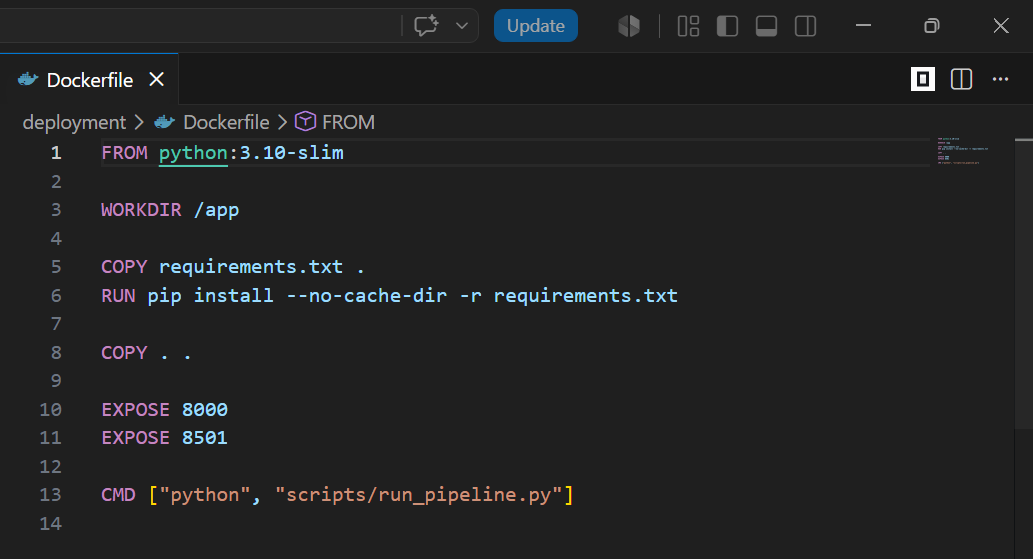
\includegraphics[width=\textwidth]{Screenshot 2026-06-27 140700.png}
    \caption{Data loading pipeline (loader.py)}\label{fig:app_loader}
\end{figure}

\section{FGSM Attack Implementation}
\label{app:fgsm}

\begin{figure}[H]
    \centering
    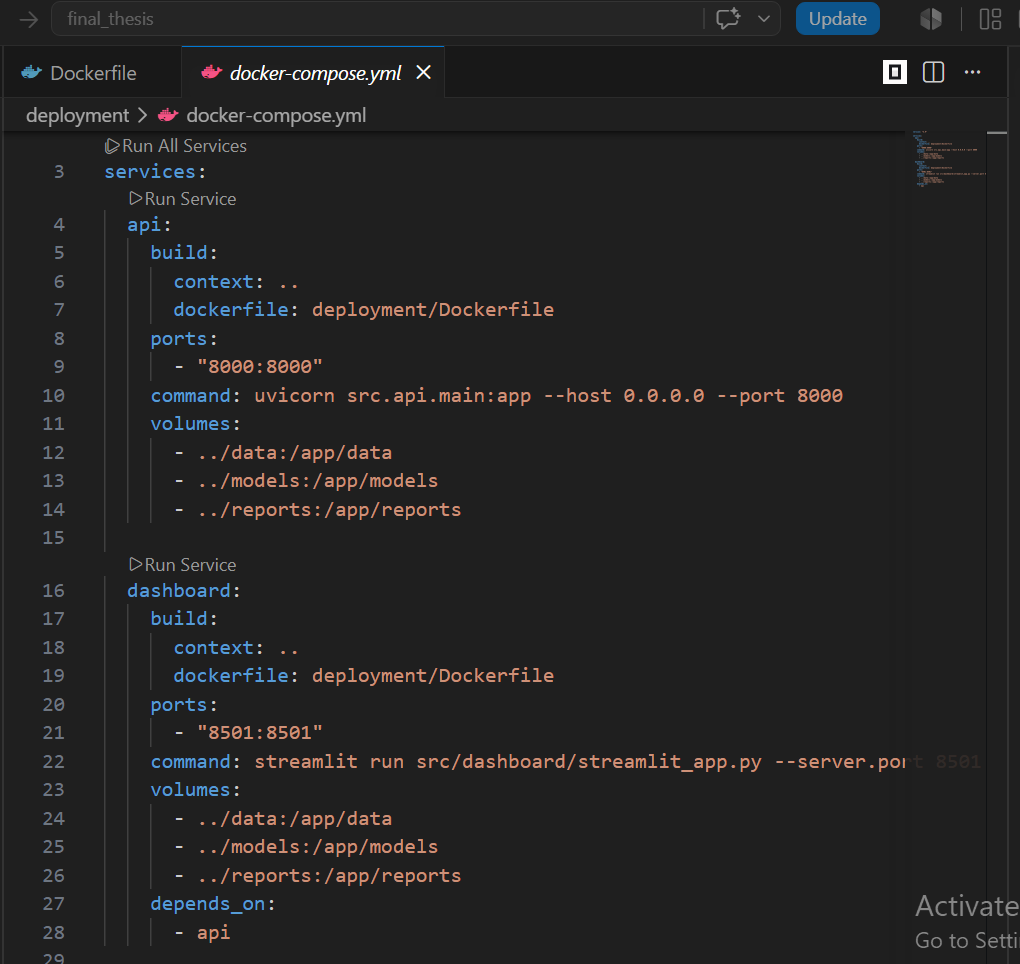
\includegraphics[width=\textwidth]{Screenshot 2026-06-27 141635.png}
    \caption{FGSM attack for tree-based models (fgsm.py)}\label{fig:app_fgsm}
\end{figure}

\section{Adversarial Training Implementation}
\label{app:advtrain}

\begin{figure}[H]
    \centering
    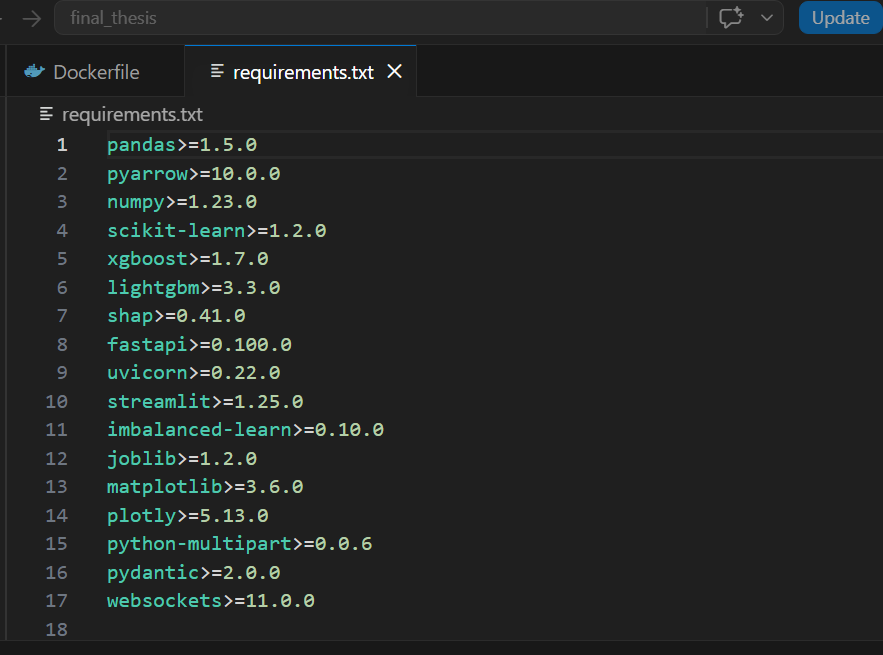
\includegraphics[width=\textwidth]{Screenshot 2026-06-27 142108.png}
    \caption{Adversarial training defense (adversarial\_training.py)}\label{fig:app_advtrain}
\end{figure}

\chapter{DEPLOYMENT CONFIGURATION}

\section{Dockerfile}

\begin{figure}[H]
    \centering
    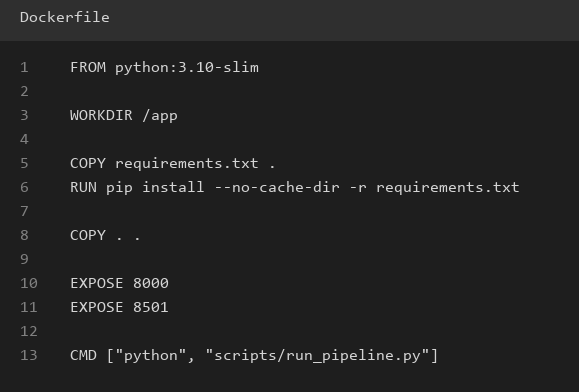
\includegraphics[width=0.85\textwidth]{dockerfile.png}
    \caption{Dockerfile for the application container}\label{fig:app_dockerfile}
\end{figure}

\section{Docker Compose}

\begin{figure}[H]
    \centering
    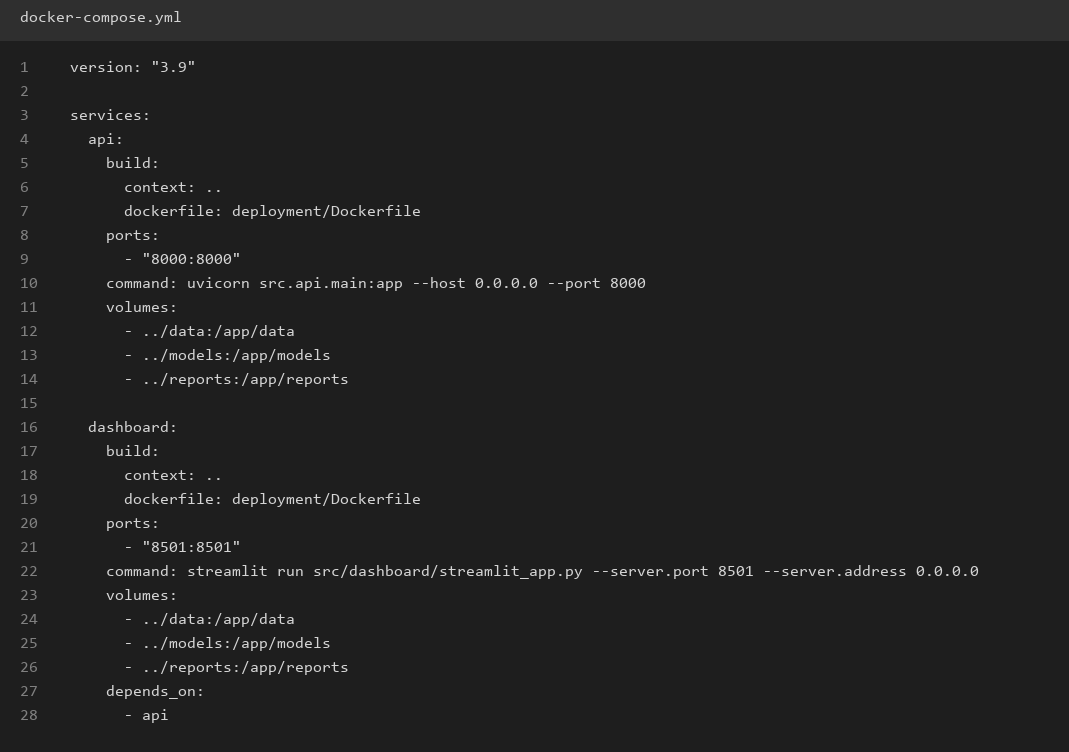
\includegraphics[width=\textwidth]{docker-compose.png}
    \caption{Docker Compose configuration for API and dashboard services}\label{fig:app_dockercompose}
\end{figure}

\section{Requirements}

\begin{figure}[H]
    \centering
    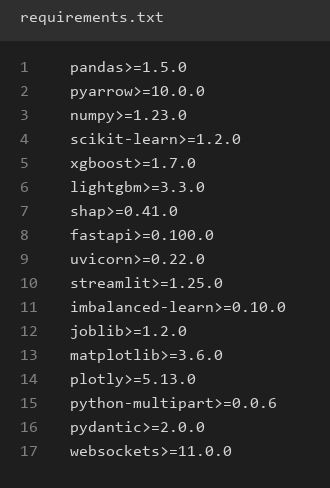
\includegraphics[width=0.85\textwidth]{requirements.png}
    \caption{Python package dependencies}\label{fig:app_requirements}
\end{figure}

\chapter{DASHBOARD SCREENSHOTS}

\begin{figure}[H]
    \centering
    \fbox{\parbox{0.8\textwidth}{\centering [Screenshot of interactive dashboard showing full pipeline results --- Insert Here]}}
    \caption{Interactive dashboard -- main view}\label{fig:dash_main}
\end{figure}

\begin{figure}[H]
    \centering
    \fbox{\parbox{0.8\textwidth}{\centering [Screenshot of dashboard showing best algorithm banner with metrics --- Insert Here]}}
    \caption{Best algorithm banner showing Accuracy, Precision, Recall, and F1}\label{fig:dash_best}
\end{figure}

\begin{figure}[H]
    \centering
    \fbox{\parbox{0.8\textwidth}{\centering [Screenshot of defense comparison section --- Insert Here]}}
    \caption{Defense comparison view}\label{fig:dash_defense}
\end{figure}

\begin{figure}[H]
    \centering
    \fbox{\parbox{0.8\textwidth}{\centering [Screenshot of SHAP explanation plots --- Insert Here]}}
    \caption{SHAP feature importance explanation}\label{fig:dash_shap}
\end{figure}

\end{appendices}

\end{document}
